\chapter{Results and Discussion}
The results of our experiments with our data set will be presented in this chapter. 30 runs of each approach that produced feasible solutions are included in the results. Note that some runs produce an infeasible solution. This due to the non-deterministic nature of metaheuristics, which will cause it to produce infeasible solutions sometimes.

\section{Environment}
All of the approaches were run in the following hardware and software configurations:

\begin{itemize}
	\item Hardware
	\begin{itemize}
		\item \textbf{CPU}: AMD Ryzen 5 5600X
		\item \textbf{GPU}: NVIDIA GeForce GTX 1050 Ti
		\item \textbf{RAM}: Crucial Ballistix RGB 3600 MHz DDR4 16 GB (8 GB x 2) CL16
	\end{itemize}
	\item Software
	\begin{itemize}
		\item \textbf{OS}: elementaryOS 5.1.7 Hera
		\item \textbf{Linux Kernel Version}: 5.4.0-99-generic
	\end{itemize}
\end{itemize}

\section{Experiments}
We have conducted two sets of experiments in order for us to evaluate the performance of our proposed GWO approach. The first set of experiments varies the GWO parameter, $c$, and the population size. It shows the impact of the parameters to the algorithm. The second set are experiments with the competing approaches. It shows how our proposed approach compares against other approaches. A population size of $50$ is used for all the experiment runs in the second set. This set will then be compared to the GWO experiment runs that have a population of the same size.

\subsection{Results with Different GWO Parameter Values}
Our proposed GWO approach only has one parameter, other than the population size, and number of iterations, the $c$ value. We used four values for the parameter: $2$, $4$, $8$, and $12$. We also varied the population size for this experiment set. The population sizes we used are: $25$, $50$, and $75$. Tables \ref{approach-gwo-c2-p25-results} to \ref{approach-gwo-c12-p75-results} show the results. We will refer to each GWO experiment as $G_{n,c}$, where $n$ is the population size, and $c$ is the value of the $c$ parameter in each experiment. So, for example, the GWO experiment with a population size of $25$ and $c = 2$ will be referred to as $G_{25,2}$, and so on. Each experiment for each parameter configuration combination has been run 30 times.

% Start of the GWO table of results for the one with a population of 25.
\begin{table}[h!]
\begin{adjustwidth}{-1.18in}{}
	\centering
	\begin{tabular}{|l|l|l|l|l|l|}
	\hline
	\multicolumn{1}{|c|}{\multirow{2}{*}{\textbf{Problem}}} & \multicolumn{5}{c|}{\textbf{GWO (c = 2, Pop. Size of 25)}} \\ \cline{2-6} 
	\multicolumn{1}{|c|}{}                                  & \multicolumn{1}{c|}{\textbf{Best}} & \multicolumn{1}{c|}{\textbf{Worst}} & \multicolumn{1}{c|}{\textbf{Avg.}} & \multicolumn{1}{c|}{\textbf{Std. Dev.}} & \multicolumn{1}{c|}{\textbf{Avg. Runtime (s)}} \\ \hline
	SFLP-II                                                 & 226.149871                                  & 328.546146                                   & 287.749326366667                      & 24.7018482581174                                 & 6.03333333333333                                  \\ \hline
	mSFLP-III                                               & 50874.238564                                & 60974.998642                                 & 55624.0061857667						         & 2544.70550235336                              & 22.4333333333333                               \\ \hline
	mKra30a                                               & 94640.759514                                & 120397.403767                                 &
	107874.742523333							&
	6706.6049593287							&
	35.9666666666667						\\ \hline
	\end{tabular}
\end{adjustwidth}
\caption{Results obtained from our proposed GWO approach with $c = 2$ and a population of $25$.}
\label{approach-gwo-c2-p25-results}
\end{table}

\begin{table}[h!]
\begin{adjustwidth}{-1.18in}{}
	\centering
	\begin{tabular}{|l|l|l|l|l|l|}
	\hline
	\multicolumn{1}{|c|}{\multirow{2}{*}{\textbf{Problem}}} & \multicolumn{5}{c|}{\textbf{GWO (c = 4, Pop. Size of 25)}} \\ \cline{2-6} 
	\multicolumn{1}{|c|}{}                                  & \multicolumn{1}{c|}{\textbf{Best}} & \multicolumn{1}{c|}{\textbf{Worst}} & \multicolumn{1}{c|}{\textbf{Avg.}} & \multicolumn{1}{c|}{\textbf{Std. Dev.}} & \multicolumn{1}{c|}{\textbf{Avg. Runtime (s)}} \\ \hline
	SFLP-II                                                 & 228.710226                                  & 373.604858                                   & 298.836421533333                      & 34.1522620177737                                 & 5.9                                  \\ \hline
	mSFLP-III                                               & 50825.278824                                & 59194.486832                                 & 55236.4286594						         & 2301.71070299619                              & 21.3333333333333                               \\ \hline
	mKra30a                                               & 87110.57618                                & 116746.599121                                 &
	104270.487286567							&
	8041.05756072353							&
	36.3333333333333						\\ \hline
	\end{tabular}
\end{adjustwidth}
\caption{Results obtained from our proposed GWO approach with $c = 4$ and a population of $25$.}
\label{approach-gwo-c4-p25-results}
\end{table}

\begin{table}[h!]
\begin{adjustwidth}{-1.18in}{}
	\centering
	\begin{tabular}{|l|l|l|l|l|l|}
	\hline
	\multicolumn{1}{|c|}{\multirow{2}{*}{\textbf{Problem}}} & \multicolumn{5}{c|}{\textbf{GWO (c = 8, Pop. Size of 25)}} \\ \cline{2-6} 
	\multicolumn{1}{|c|}{}                                  & \multicolumn{1}{c|}{\textbf{Best}} & \multicolumn{1}{c|}{\textbf{Worst}} & \multicolumn{1}{c|}{\textbf{Avg.}} & \multicolumn{1}{c|}{\textbf{Std. Dev.}} & \multicolumn{1}{c|}{\textbf{Avg. Runtime (s)}} \\ \hline
	SFLP-II                                                 & 249.624192                                  & 368.435807                                   & 313.640670633333                     & 29.7958232730557                                 & 6.23333333333333                                  \\ \hline
	mSFLP-III                                               & 51250.638187                                & 57894.186882                                 & 54206.6467008333						         & 1334.40810225102                              & 23.6                               \\ \hline
	mKra30a                                               & 95254.061554                                & 118719.490257                                 &
	105760.743434367							&
	6557.69877516131							&
	37.0666666666667						\\ \hline
	\end{tabular}
\end{adjustwidth}
\caption{Results obtained from our proposed GWO approach with $c = 8$ and a population of $25$.}
\label{approach-gwo-c8-p25-results}
\end{table}

\begin{table}[h!]
\begin{adjustwidth}{-1.18in}{}
	\centering
	\begin{tabular}{|l|l|l|l|l|l|}
	\hline
	\multicolumn{1}{|c|}{\multirow{2}{*}{\textbf{Problem}}} & \multicolumn{5}{c|}{\textbf{GWO (c = 12, Pop. Size of 25)}} \\ \cline{2-6} 
	\multicolumn{1}{|c|}{}                                  & \multicolumn{1}{c|}{\textbf{Best}} & \multicolumn{1}{c|}{\textbf{Worst}} & \multicolumn{1}{c|}{\textbf{Avg.}} & \multicolumn{1}{c|}{\textbf{Std. Dev.}} & \multicolumn{1}{c|}{\textbf{Avg. Runtime (s)}} \\ \hline
	SFLP-II                                                 & 255.639347                                  & 358.033844                                   & 315.207093933333                      & 26.4399229476443                                 & 6.36666666666667                                  \\ \hline
	mSFLP-III                                               & 51328.437737                                & 62758.004044                                 & 55331.2312675333						         & 2540.54370041386                              & 21.2333333333333                              \\ \hline
	mKra30a                                               & 93525.765816                                & 124181.531029                                 &
	108251.9895637							&
	8151.19724950765							&
	37.3						\\ \hline
	\end{tabular}
\end{adjustwidth}
\caption{Results obtained from our proposed GWO approach with $c = 12$ and a population of $25$.}
\label{approach-gwo-c12-p25-results}
\end{table}

% Start of the GWO table of results for the one with a population of 50.
\begin{table}[h!]
	\begin{adjustwidth}{-1.18in}{}
		\centering
		\begin{tabular}{|l|l|l|l|l|l|}
			\hline
			\multicolumn{1}{|c|}{\multirow{2}{*}{\textbf{Problem}}} & \multicolumn{5}{c|}{\textbf{GWO (c = 2, Pop. Size of 50)}} \\ \cline{2-6} 
			\multicolumn{1}{|c|}{}                                  & \multicolumn{1}{c|}{\textbf{Best}} & \multicolumn{1}{c|}{\textbf{Worst}} & \multicolumn{1}{c|}{\textbf{Avg.}} & \multicolumn{1}{c|}{\textbf{Std. Dev.}} & \multicolumn{1}{c|}{\textbf{Avg. Runtime (s)}} \\ \hline
			SFLP-II                                                 & 221.18019                                  & 341.568304                                   & 283.795019233333                      & 28.9742518867792                                 & 13.2666666666667                                  \\ \hline
			mSFLP-III                                               & 47597.794662                                & 62827.738159                                 & 54495.2676476667						         & 3328.18744058766                              & 40.1333333333333                               \\ \hline
			mKra30a                                               & 88657.824898                                & 121124.59779                                 &
			102742.1803823							&
			7156.18271087496							&
			73.3333333333333						\\ \hline
		\end{tabular}
	\end{adjustwidth}
	\caption{Results obtained from our proposed GWO approach with $c = 2$ and a population of $50$.}
	\label{approach-gwo-c2-p50-results}
\end{table}

\begin{table}[h!]
	\begin{adjustwidth}{-1.18in}{}
		\centering
		\begin{tabular}{|l|l|l|l|l|l|}
			\hline
			\multicolumn{1}{|c|}{\multirow{2}{*}{\textbf{Problem}}} & \multicolumn{5}{c|}{\textbf{GWO (c = 4, Pop. Size of 50)}} \\ \cline{2-6} 
			\multicolumn{1}{|c|}{}                                  & \multicolumn{1}{c|}{\textbf{Best}} & \multicolumn{1}{c|}{\textbf{Worst}} & \multicolumn{1}{c|}{\textbf{Avg.}} & \multicolumn{1}{c|}{\textbf{Std. Dev.}} & \multicolumn{1}{c|}{\textbf{Avg. Runtime (s)}} \\ \hline
			SFLP-II                                                 & 241.862298                                  & 389.711568                                   & 294.2461242                      & 33.7641257773172                                 & 13.1333333333333                                  \\ \hline
			mSFLP-III                                               & 50250.080536                                & 57916.673454                                 & 53421.9267731333						         & 2239.06725435468                              & 41.9666666666667                               \\ \hline
			mKra30a                                               & 90599.06601                                & 122300.269909                                 &
			102855.4831497							&
			8820.10238434929							&
			70.9666666666667						\\ \hline
		\end{tabular}
	\end{adjustwidth}
	\caption{Results obtained from our proposed GWO approach with $c = 4$ and a population of $50$.}
	\label{approach-gwo-c4-p50-results}
\end{table}

\begin{table}[h!]
	\begin{adjustwidth}{-1.18in}{}
		\centering
		\begin{tabular}{|l|l|l|l|l|l|}
			\hline
			\multicolumn{1}{|c|}{\multirow{2}{*}{\textbf{Problem}}} & \multicolumn{5}{c|}{\textbf{GWO (c = 8, Pop. Size of 50)}} \\ \cline{2-6} 
			\multicolumn{1}{|c|}{}                                  & \multicolumn{1}{c|}{\textbf{Best}} & \multicolumn{1}{c|}{\textbf{Worst}} & \multicolumn{1}{c|}{\textbf{Avg.}} & \multicolumn{1}{c|}{\textbf{Std. Dev.}} & \multicolumn{1}{c|}{\textbf{Avg. Runtime (s)}} \\ \hline
			SFLP-II                                                 & 240.638127                                  & 413.077936                                   & 299.553292466667                     & 40.469222577263                                 & 12.7333333333333                                  \\ \hline
			mSFLP-III                                               & 48844.175789                                & 59710.615997                                 & 52699.5983075667						         & 2062.76885562279                              & 41.2666666666667                               \\ \hline
			mKra30a                                               & 84929.672058                                & 112251.415863                                 &
			101570.163644533							&
			6490.61277032704							&
			72.1						\\ \hline
		\end{tabular}
	\end{adjustwidth}
	\caption{Results obtained from our proposed GWO approach with $c = 8$ and a population of $50$.}
	\label{approach-gwo-c8-p50-results}
\end{table}

\begin{table}[h!]
	\begin{adjustwidth}{-1.18in}{}
		\centering
		\begin{tabular}{|l|l|l|l|l|l|}
			\hline
			\multicolumn{1}{|c|}{\multirow{2}{*}{\textbf{Problem}}} & \multicolumn{5}{c|}{\textbf{GWO (c = 12, Pop. Size of 50)}} \\ \cline{2-6} 
			\multicolumn{1}{|c|}{}                                  & \multicolumn{1}{c|}{\textbf{Best}} & \multicolumn{1}{c|}{\textbf{Worst}} & \multicolumn{1}{c|}{\textbf{Avg.}} & \multicolumn{1}{c|}{\textbf{Std. Dev.}} & \multicolumn{1}{c|}{\textbf{Avg. Runtime (s)}} \\ \hline
			SFLP-II                                                 & 261.869799                                  & 381.586061                                   & 315.831642166667                      & 31.7204847308938                                 & 13.6666666666667                                  \\ \hline
			mSFLP-III                                               & 48920.979538                                & 56477.689476                                 & 52837.3591700333						         & 1980.22102755171                              & 42.2333333333333                              \\ \hline
			mKra30a                                               & 92563.720146                                & 128598.716599                                 &
			105348.4949903							&
			9267.72959691125							&
			69.5666666666667						\\ \hline
		\end{tabular}
	\end{adjustwidth}
	\caption{Results obtained from our proposed GWO approach with $c = 12$ and a population of $50$.}
	\label{approach-gwo-c12-p50-results}
\end{table}

% Start of the GWO table of results for the one with a population of 75.
\begin{table}[h!]
	\begin{adjustwidth}{-1.18in}{}
		\centering
		\begin{tabular}{|l|l|l|l|l|l|}
			\hline
			\multicolumn{1}{|c|}{\multirow{2}{*}{\textbf{Problem}}} & \multicolumn{5}{c|}{\textbf{GWO (c = 2, Pop. Size of 75)}} \\ \cline{2-6} 
			\multicolumn{1}{|c|}{}                                  & \multicolumn{1}{c|}{\textbf{Best}} & \multicolumn{1}{c|}{\textbf{Worst}} & \multicolumn{1}{c|}{\textbf{Avg.}} & \multicolumn{1}{c|}{\textbf{Std. Dev.}} & \multicolumn{1}{c|}{\textbf{Avg. Runtime (s)}} \\ \hline
			SFLP-II                                                 & 205.666955                                  & 386.356476                                   & 290.063388433333                      & 38.0436802516604                                 & 18.8666666666667                                  \\ \hline
			mSFLP-III                                               & 50179.684898                                & 57659.66436                                 & 54015.3749653						         & 2050.7167136713                              & 61.1                               \\ \hline
			mKra30a                                               & 88740.484344                                & 117173.305939                                 &
			99149.0616948							&
			5833.24082935413							&
			104.7						\\ \hline
		\end{tabular}
	\end{adjustwidth}
	\caption{Results obtained from our proposed GWO approach with $c = 2$ and a population of $75$.}
	\label{approach-gwo-c2-p75-results}
\end{table}

\begin{table}[h!]
	\begin{adjustwidth}{-1.18in}{}
		\centering
		\begin{tabular}{|l|l|l|l|l|l|}
			\hline
			\multicolumn{1}{|c|}{\multirow{2}{*}{\textbf{Problem}}} & \multicolumn{5}{c|}{\textbf{GWO (c = 4, Pop. Size of 75)}} \\ \cline{2-6} 
			\multicolumn{1}{|c|}{}                                  & \multicolumn{1}{c|}{\textbf{Best}} & \multicolumn{1}{c|}{\textbf{Worst}} & \multicolumn{1}{c|}{\textbf{Avg.}} & \multicolumn{1}{c|}{\textbf{Std. Dev.}} & \multicolumn{1}{c|}{\textbf{Avg. Runtime (s)}} \\ \hline
			SFLP-II                                                 & 239.258536                                  & 406.790997                                   & 302.005947566667                      & 39.1344289013742                                 & 18.9                                  \\ \hline
			mSFLP-III                                               & 48752.443314                                & 56156.624268                                 & 52037.6629276						         & 2313.4004317195                              & 61.5333333333333                               \\ \hline
			mKra30a                                               & 89197.608078                                & 121878.61042                                 &
			99482.2352776							&
			7069.6968084522							&
			107.966666666667						\\ \hline
		\end{tabular}
	\end{adjustwidth}
	\caption{Results obtained from our proposed GWO approach with $c = 4$ and a population of $75$.}
	\label{approach-gwo-c4-p75-results}
\end{table}

\begin{table}[h!]
	\begin{adjustwidth}{-1.18in}{}
		\centering
		\begin{tabular}{|l|l|l|l|l|l|}
			\hline
			\multicolumn{1}{|c|}{\multirow{2}{*}{\textbf{Problem}}} & \multicolumn{5}{c|}{\textbf{GWO (c = 8, Pop. Size of 75)}} \\ \cline{2-6} 
			\multicolumn{1}{|c|}{}                                  & \multicolumn{1}{c|}{\textbf{Best}} & \multicolumn{1}{c|}{\textbf{Worst}} & \multicolumn{1}{c|}{\textbf{Avg.}} & \multicolumn{1}{c|}{\textbf{Std. Dev.}} & \multicolumn{1}{c|}{\textbf{Avg. Runtime (s)}} \\ \hline
			SFLP-II                                                 & 246.916627                                  & 393.744452                                   & 309.957982766667                     & 32.0156308267039                                 & 19.5                                  \\ \hline
			mSFLP-III                                               & 49276.248596                                & 54977.558044                                 & 51801.8837937333						         & 1419.1918023338                              & 63.0333333333333                               \\ \hline
			mKra30a                                               & 87299.715054                                & 113760.078079                                 &
			98968.6223121							&
			6443.60722715266							&
			108.7						\\ \hline
		\end{tabular}
	\end{adjustwidth}
	\caption{Results obtained from our proposed GWO approach with $c = 8$ and a population of $75$.}
	\label{approach-gwo-c8-p75-results}
\end{table}

\begin{table}[h!]
	\begin{adjustwidth}{-1.18in}{}
		\centering
		\begin{tabular}{|l|l|l|l|l|l|}
			\hline
			\multicolumn{1}{|c|}{\multirow{2}{*}{\textbf{Problem}}} & \multicolumn{5}{c|}{\textbf{GWO (c = 12, Pop. Size of 75)}} \\ \cline{2-6} 
			\multicolumn{1}{|c|}{}                                  & \multicolumn{1}{c|}{\textbf{Best}} & \multicolumn{1}{c|}{\textbf{Worst}} & \multicolumn{1}{c|}{\textbf{Avg.}} & \multicolumn{1}{c|}{\textbf{Std. Dev.}} & \multicolumn{1}{c|}{\textbf{Avg. Runtime (s)}} \\ \hline
			SFLP-II                                                 & 243.386427                                  & 413.874466                                   & 307.3213231                      & 36.2239957721235                                 & 19.3333333333333                                  \\ \hline
			mSFLP-III                                               & 49644.232903                                & 55524.684891                                 & 51837.8766529667						         & 1430.57988385005                              & 61.7666666666667                              \\ \hline
			mKra30a                                               & 86942.304199                                & 108422.175175                                 &
			98108.9092933667							&
			6511.43059062118							&
			111.266666666667						\\ \hline
		\end{tabular}
	\end{adjustwidth}
	\caption{Results obtained from our proposed GWO approach with $c = 12$ and a population of $75$.}
	\label{approach-gwo-c12-p75-results}
\end{table}

Let us first discuss the results with the SFLP-II problem. Table \ref{full-data-gwo-sflp-ii} provides a summary of the results of the experiments performed for the problem using the GWO approach. Figure \ref{approach-gwo-sflp-ii-average-fitness-as-c-value-increases}, on the other hand, shows a line graph that displays the average fitness of solutions of each population size when solving the SFLP-II problem as the $c$ value increases. For the problem, $G_{50,2}$ has the best average compared to the other configurations with a value of $283.795019233333$. The worst average belonged to $G_{50,12}$ with a value of $315.831642166667$. The configuration with the best solution produced would be $G_{75,2}$ with the solution having a value of $205.666955$. Figure \ref{approach-gwo-sflp-ii-best-solution-fitness-over-time} shows the progress of the solution as the number of iterations increase. On the other hand, the worst solution was produced by $G_{75,12}$ with a value of $413.874466$. Figure \ref{approach-gwo-sflp-ii-best-and-worst-solutions-visualization} shows what these solutions look like. The average runtime of the experiments increase as the population size increases. In a similar fashion, the experiments with population sizes of $25$ and $50$, their average fitness value worsens (increases) as the value of $c$ increases. However, with a population size of $75$, the same trend is reflected until $c = 12$, where the average fitness improves.

\begin{figure}[h!]
\centering
\begin{adjustwidth}{-0.45in}{}
	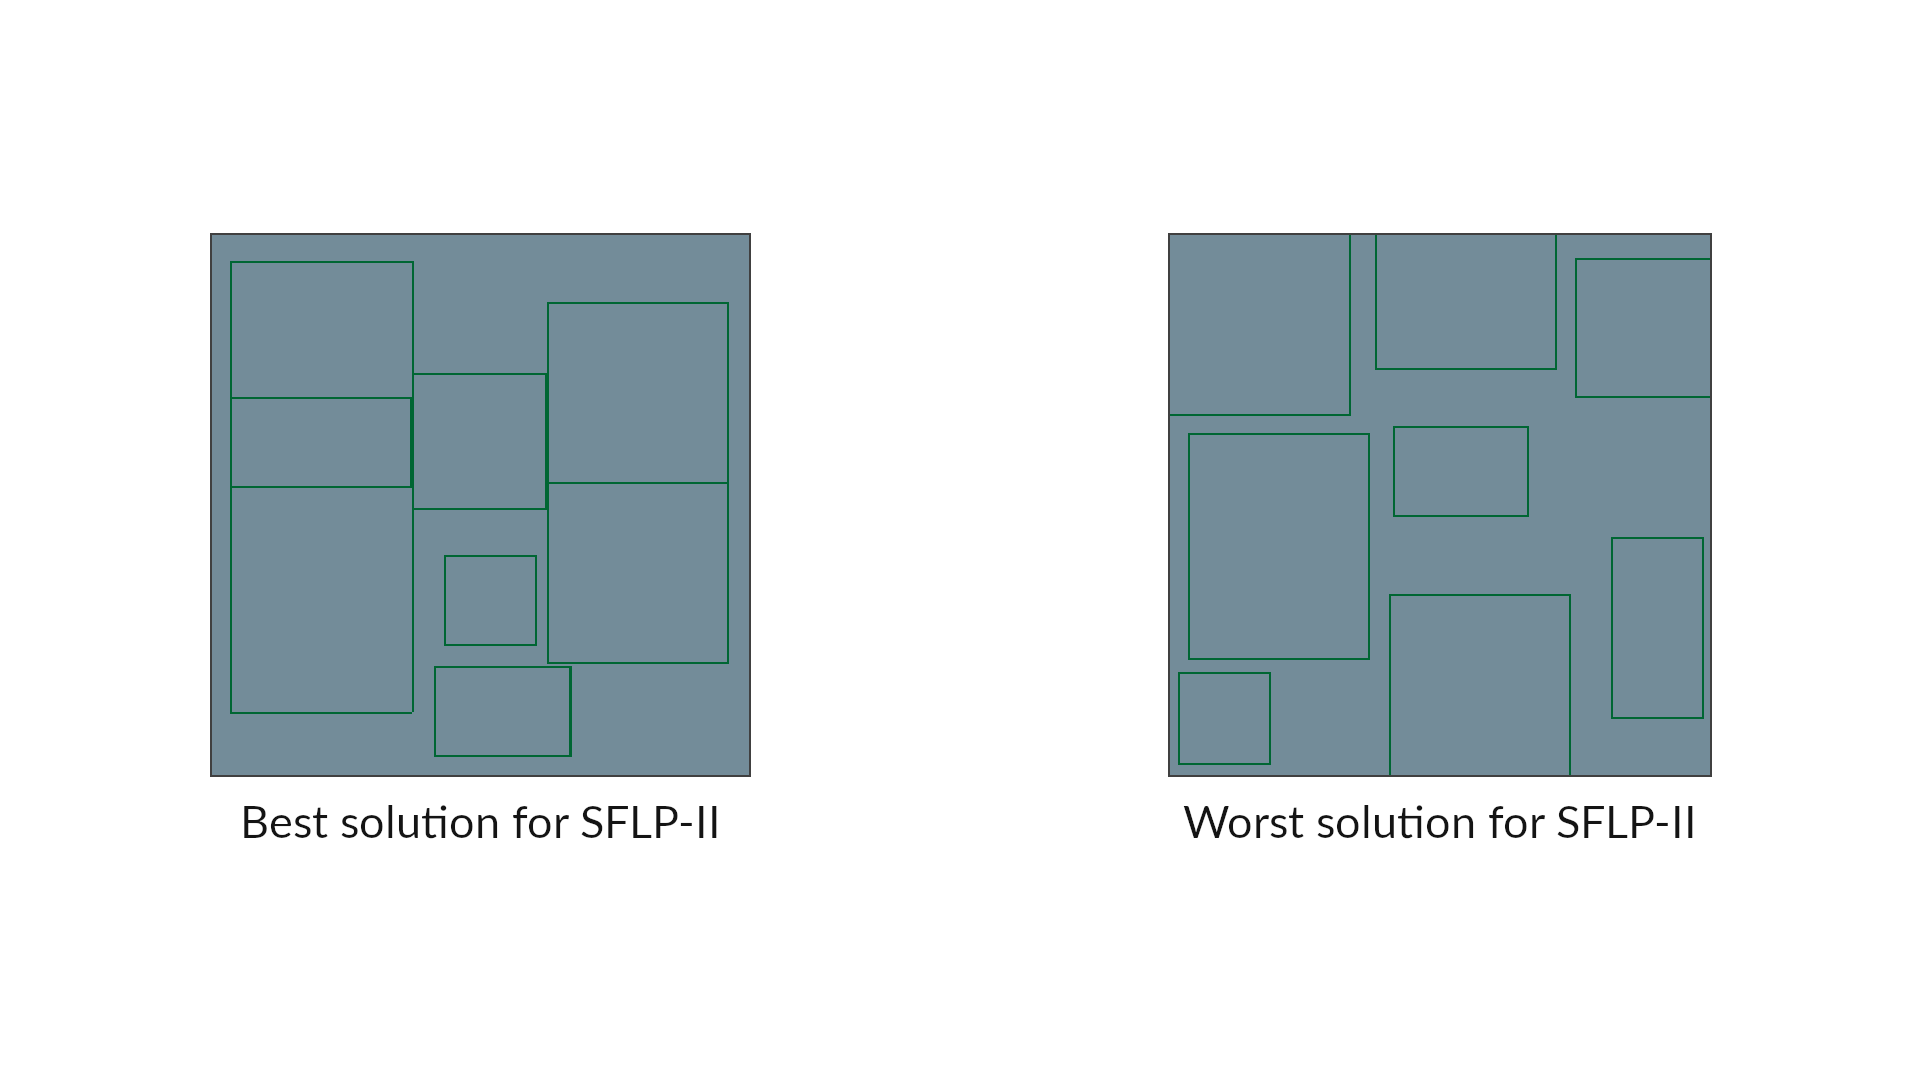
\includegraphics[scale=1.0]{./images/chap07-rd/gwo-sflp2-best-and-worst-solutions.png}
\end{adjustwidth}
\caption{Visualizations of the best and worst solutions generated by our GWO approach for the SFLP-II problem. The best solution was generated by $G_{75,2}$, and the worst generated by $G_{75,12}$.}
\label{approach-gwo-sflp-ii-best-and-worst-solutions-visualization}
\end{figure}

\begin{figure}[h!]
\centering
\begin{adjustwidth}{-0.45in}{}
	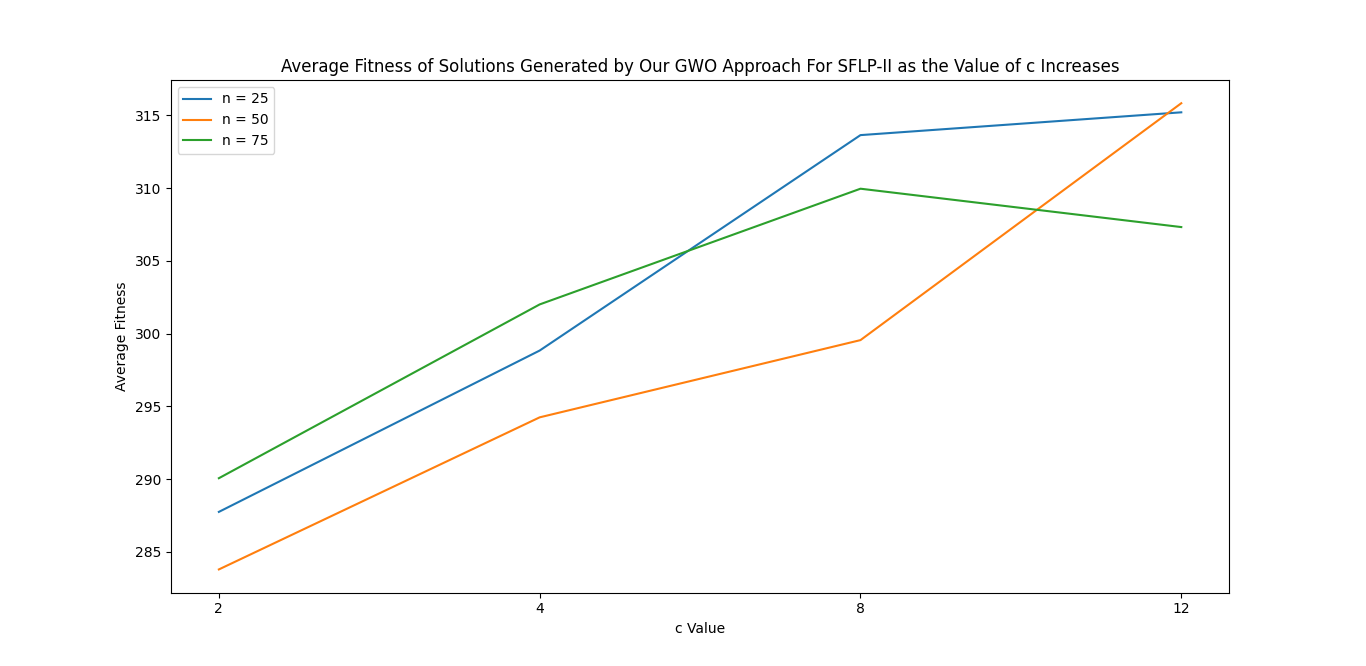
\includegraphics[scale=0.5]{./images/chap07-rd/gwo-only-sflp2-average-fitness-as-c-value-increases.png}
\end{adjustwidth}
\caption{The average fitness of the solutions produced by our GWO approach as the $c$ value increases when solving the SFLP-II problem. Each line uses a different population with the blue line representing experiments using a population size ($n$) of 25, the yellow lines representing those with $n = 50$, and the green lines representing those with $n = 75$.}
\label{approach-gwo-sflp-ii-average-fitness-as-c-value-increases}
\end{figure}

\begin{figure}[h!]
\centering
\begin{adjustwidth}{-0.45in}{}
	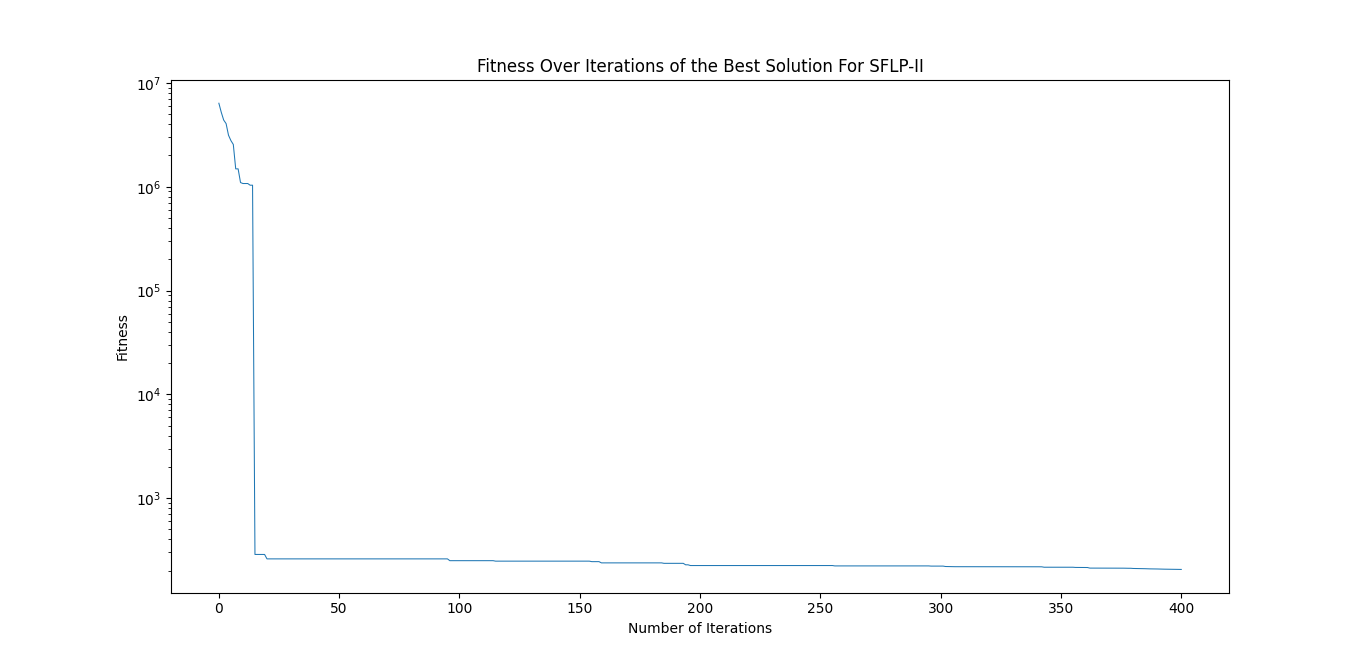
\includegraphics[scale=0.5]{./images/chap07-rd/gwo-only-sflp2-best-solution-fitness-graph.png}
\end{adjustwidth}
\caption{The fitness of the best solution generated by $G_{75,2}$ as the number of iterations increase while solving the SFLP-II problem.}
\label{approach-gwo-sflp-ii-best-solution-fitness-over-time}
\end{figure}

As with the mSFLP-III problem, of which Table \ref{full-data-gwo-msflp-iii} provides the summary of the experimental results, the best average was produced by $G_{75,8}$ with a value of $51801.8837937333$. $G_{25,2}$ produced the worst average with a value of $55624.0061857667$. For this problem, the best solution produced has a fitness of $47597.794662$, and is generated by $G_{50,2}$. Figure \ref{approach-gwo-msflp-iii-best-solution-fitness-over-time} shows the progress of this solution as the number of iterations increase. Interestingly, $G_{50,2}$ has also generated the worst solution with a fitness value of $62827.738159$. These solutions are visualized by Figure \ref{approach-gwo-msflp-iii-best-and-worst-solutions-visualization}. Parallel to the observed behaviour with the SFLP-II problem, the average runtime of the experiments also increases as the size of the population increases. A trend is also observable as the $c$ value increase that applies to all population sizes used. Increasing the $c$ value shows an improvement in the fitness value (value decreases). Unfortunately, this behaviour changes when $c = 12$, where the fitness worsens. To supplement Table \ref{full-data-gwo-msflp-iii}, we are also providing Figure \ref{approach-gwo-msflp-iii-average-fitness-as-c-value-increases}, which presents a line graph version of the results displaying the relationship between the $c$ value and the average fitness of the experiments solving the problem in every population size we are using.

\begin{figure}[h!]
\centering
\begin{adjustwidth}{-0.45in}{}
	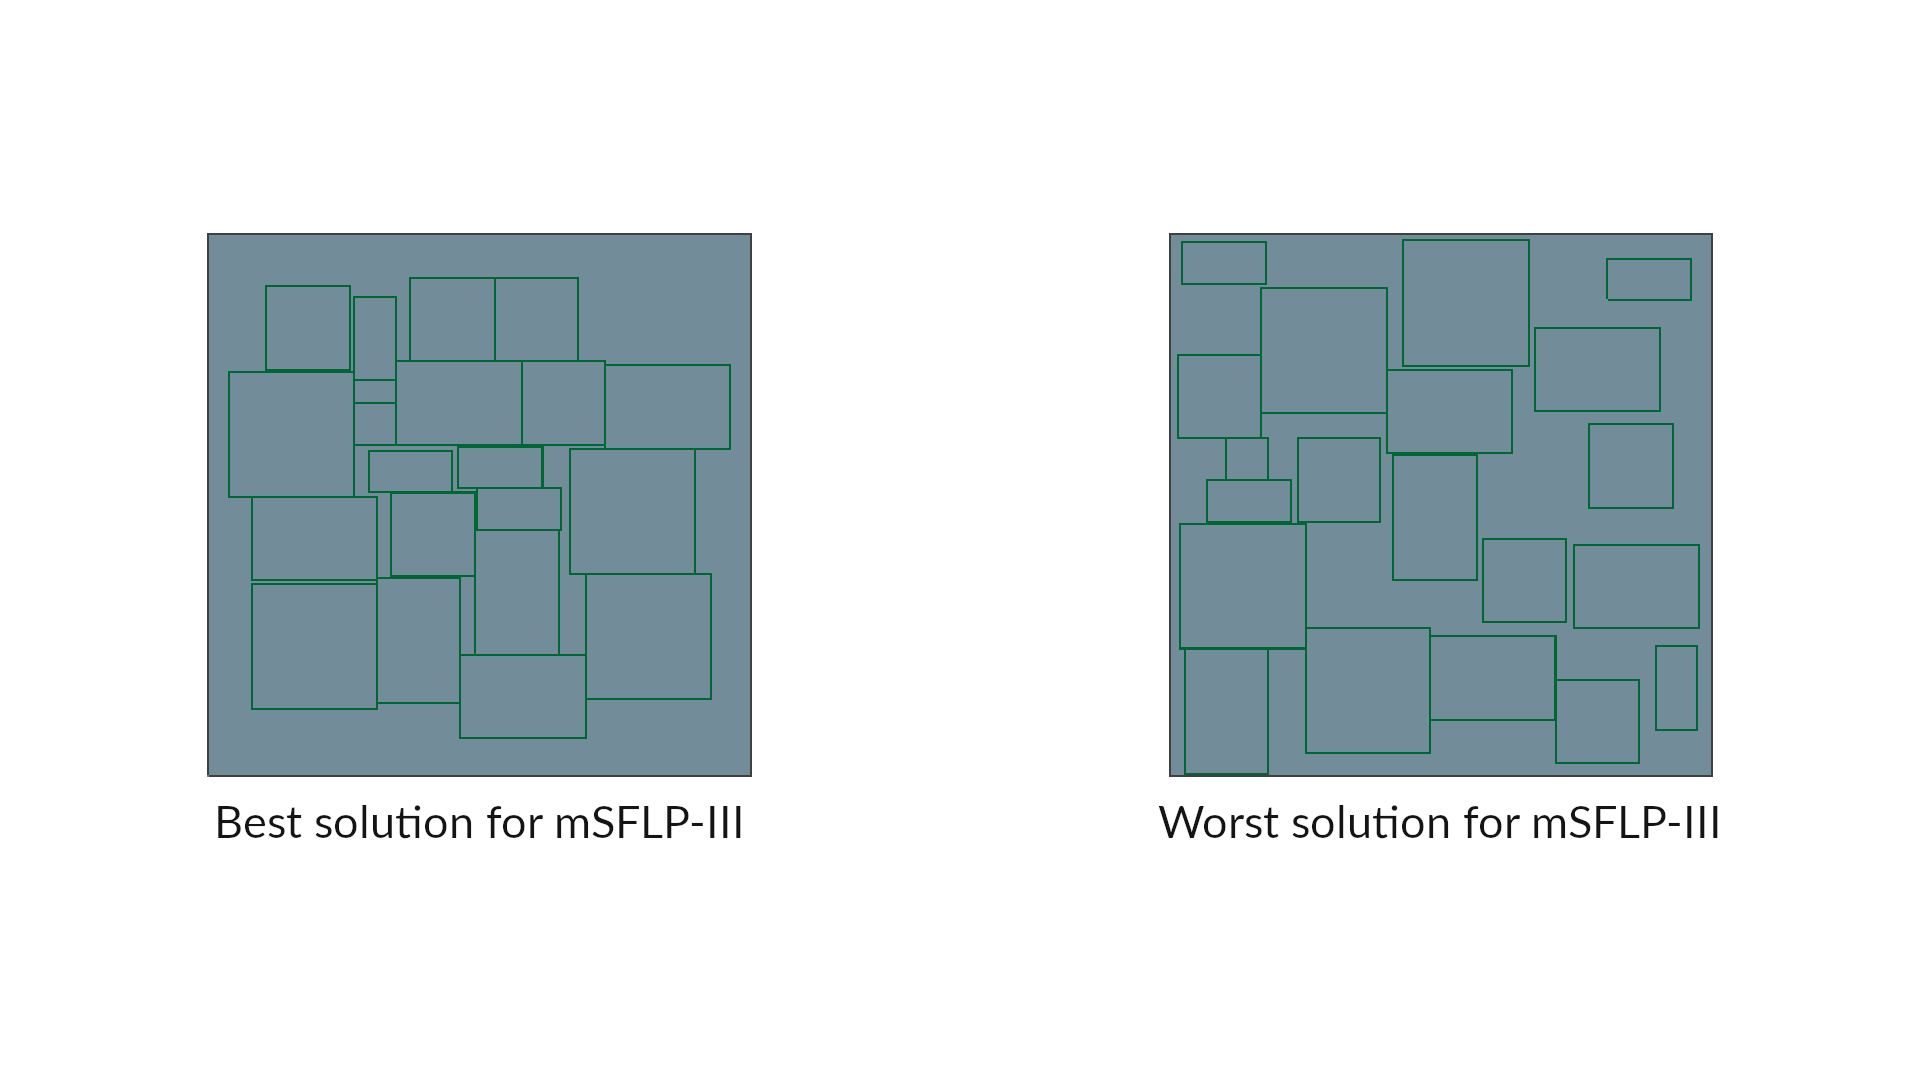
\includegraphics[scale=1.0]{./images/chap07-rd/gwo-msflp-iii-best-and-worst-solutions.png}
\end{adjustwidth}
\caption{Visualizations of the best and worst solutions generated by our GWO approach for the mSFLP-III problem. The best and worst solutions were generated by $G_{50,2}$.}
\label{approach-gwo-msflp-iii-best-and-worst-solutions-visualization}
\end{figure}

\begin{figure}[h!]
\centering
\begin{adjustwidth}{-0.45in}{}
	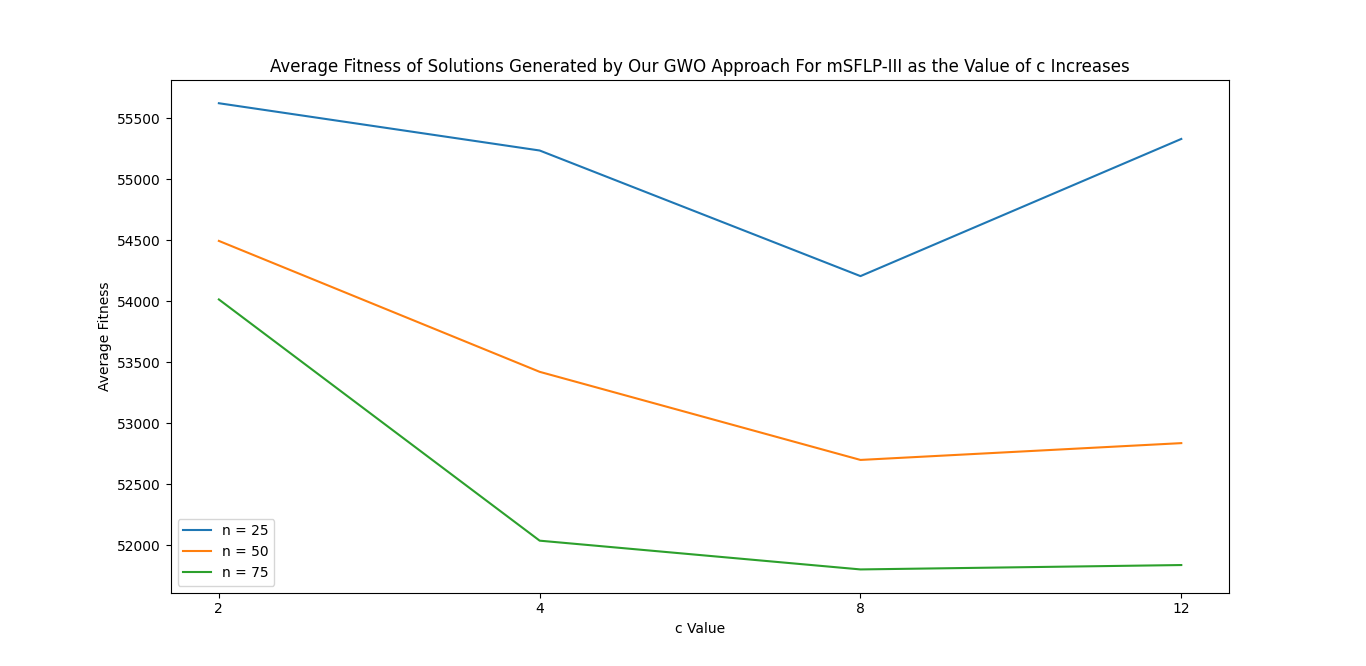
\includegraphics[scale=0.5]{./images/chap07-rd/gwo-only-msflp3-average-fitness-as-c-value-increases.png}
\end{adjustwidth}
\caption{The average fitness of the solutions produced by our GWO approach as the $c$ value increases when solving the mSFLP-III problem. Each line uses a different population with the blue line representing experiments using a population size ($n$) of 25, the yellow lines representing those with $n = 50$, and the green lines representing those with $n = 75$.}
\label{approach-gwo-msflp-iii-average-fitness-as-c-value-increases}
\end{figure}

\begin{figure}[h!]
\centering
\begin{adjustwidth}{-0.45in}{}
	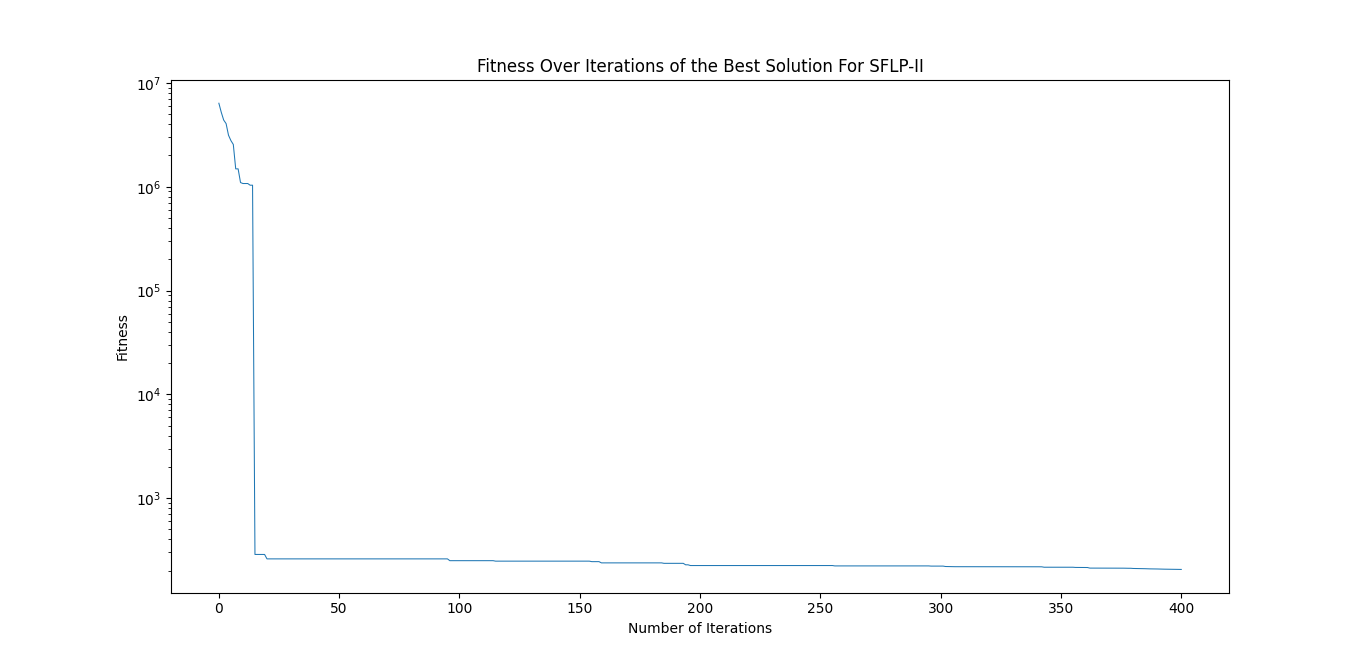
\includegraphics[scale=0.5]{./images/chap07-rd/gwo-only-sflp2-best-solution-fitness-graph.png}
\end{adjustwidth}
\caption{The fitness of the best solution generated by $G_{50,2}$ as the number of iterations increasee while solving the mSFLP-III problem.}
\label{approach-gwo-msflp-iii-best-solution-fitness-over-time}
\end{figure}

Lastly, we present a brief overview of the results we obtained for the mKra30a problem. Table \ref{full-data-gwo-mkra30a} shows the summary of the experimental results for the problem, and Figure \ref{approach-gwo-mkra30a-average-fitness-as-c-value-increases} provides a graph version of the results showcasing the impact of the value of $c$ on the average fitness of the experiments solving the problem for each population size we are using. The best average for this problem was produced by $G_{75,12}$ with a value of $98108.9092933667$. On the contrary, the worst average was produced by $G_{25,12}$ with a value of $108251.9895637$. The best solution has a fitness value of $84929.672058$, and is generated by $G_{50,8}$. Figure \ref{approach-gwo-mkra30a-best-solution-fitness-over-time} shows its progress over iterations as it solves the mKra30a problem. The worse solution, on the other hand, with a value of $128598.716599$, was produced by $G_{50,12}$. These solutions are visualized by Figure \ref{approach-gwo-mkra30a-best-and-worst-solutions-visualization}. In the same vein as the two aforementioned problems, the average runtime of the experiments increase as the population size increased. As for the values of the average fitness values with respect to the population size and $c$ values, no common trend can be observed for the three different population sizes, unlike with the previous problems. Problems with population sizes of $50$ and $75$ share a common trend from $c = 2$ to $c = 8$, where the increasing the $c$ value first worsens the average fitness, but the fitness then improves. However, when increasing the $c$ value from $8$ to $12$, the behaviour differs. With a population size of $50$, the average fitness worsens. On the other hand, with a population size of $75$, the average fitness improves instead. Lastly, the configuration with a population size of $25$ acts differently from the configurations with the aforementioned population sizes. With a population size of $25$, the average fitness value when increasing the $c$ value from $2$ to $4$ initially shows an improvement of the average fitness. However, increasing the $c$ value further results in worsening average fitness values.

\begin{figure}[h!]
\centering
\begin{adjustwidth}{-0.45in}{}
	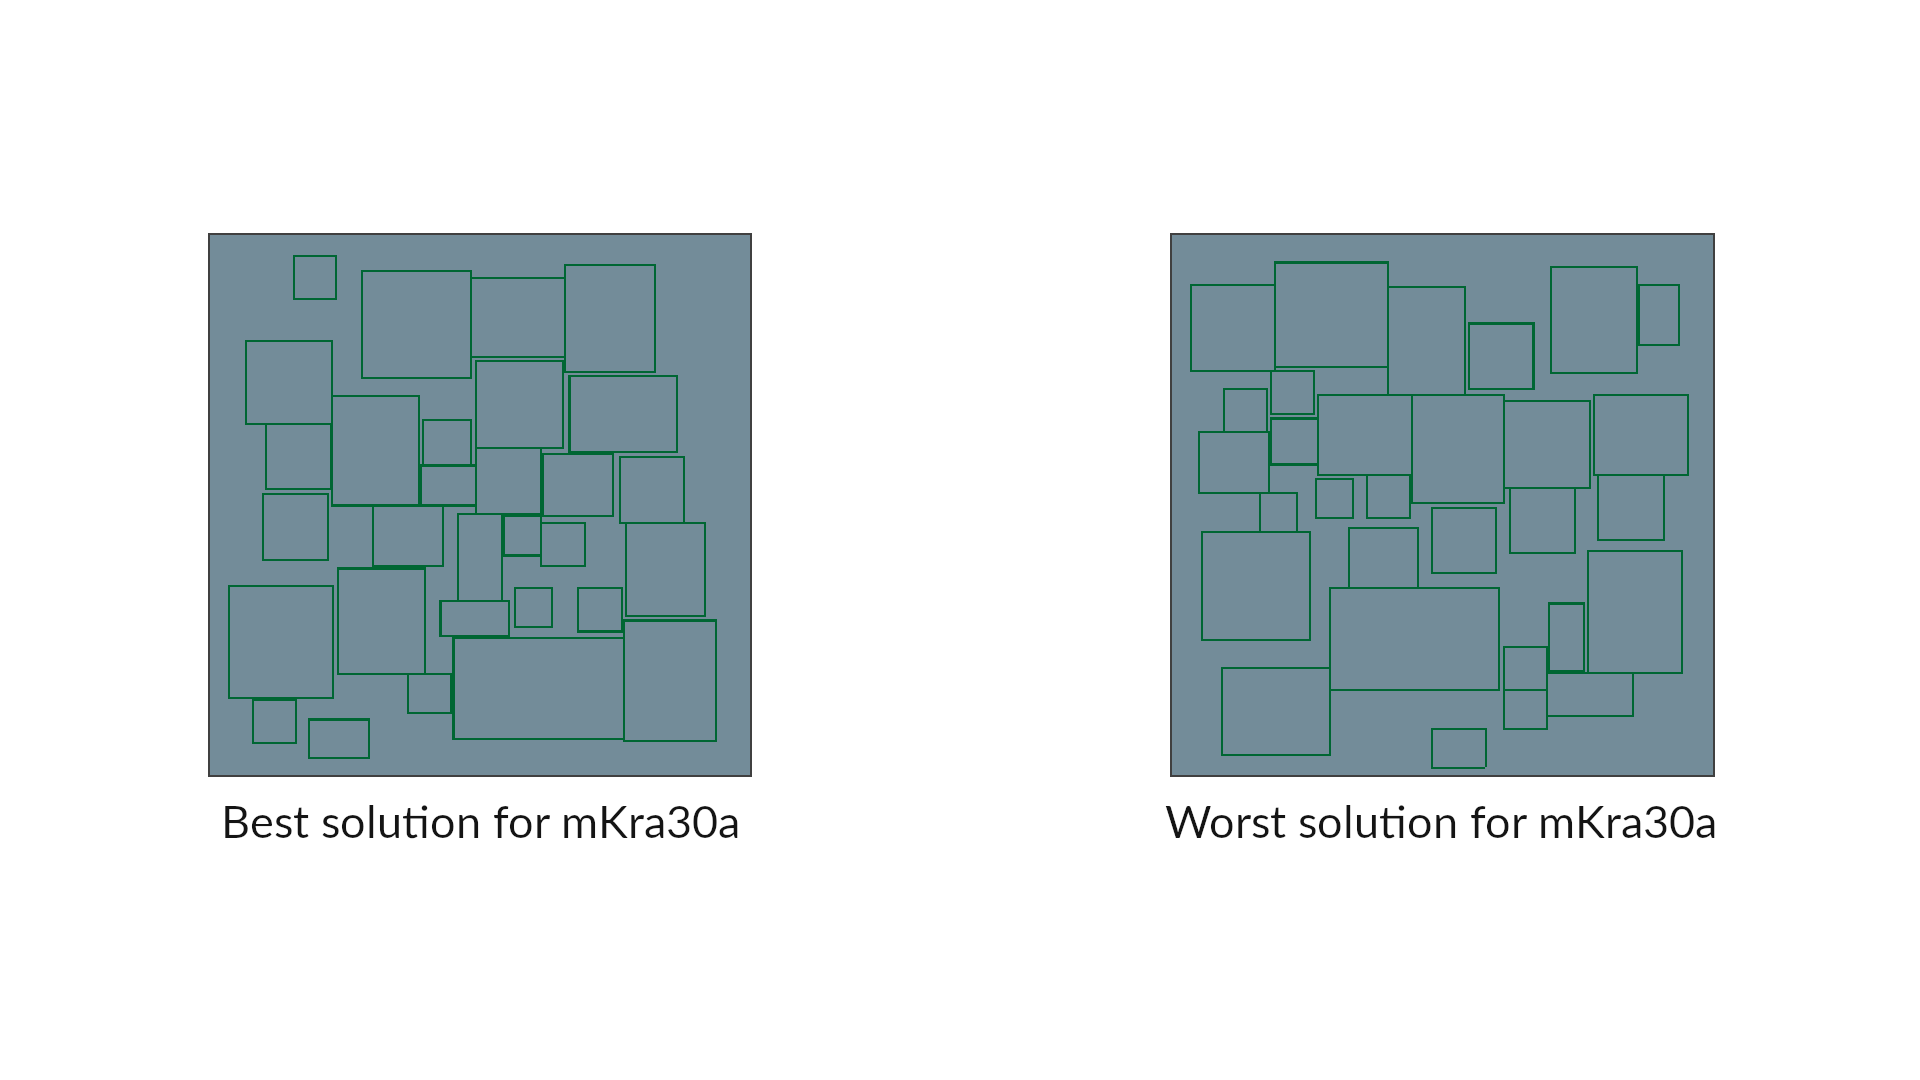
\includegraphics[scale=1.0]{./images/chap07-rd/gwo-mkra30a-best-and-worst-solutions.png}
\end{adjustwidth}
\caption{Visualizations of the best and worst solutions generated by our GWO approach for the mKra30a problem. The best solution was generated by $G_{50,8}$, with the worst generated by $G_{50,12}$.}
\label{approach-gwo-mkra30a-best-and-worst-solutions-visualization}
\end{figure}

\begin{figure}[h!]
\centering
\begin{adjustwidth}{-0.45in}{}
	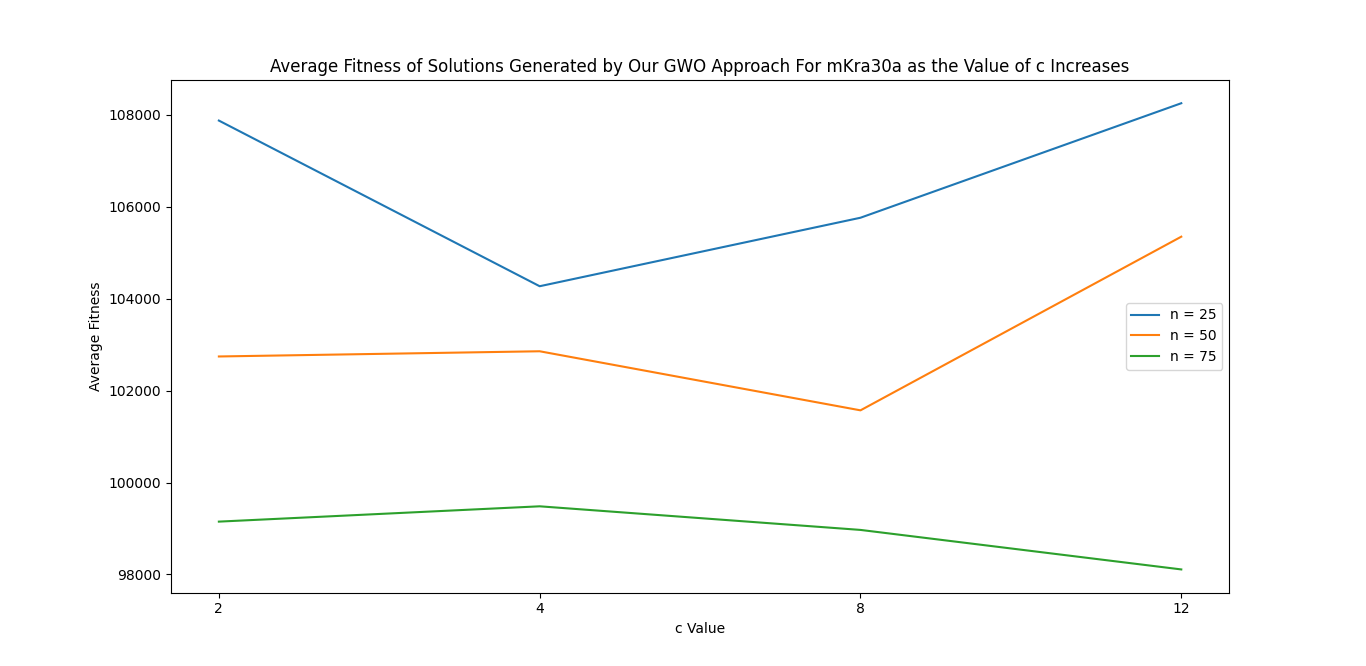
\includegraphics[scale=0.5]{./images/chap07-rd/gwo-only-mkra30a-average-fitness-as-c-value-increases.png}
\end{adjustwidth}
\caption{The average fitness of the solutions produced by our GWO approach as the $c$ value increases when solving the mKra30a problem. Each line uses a different population with the blue line representing experiments using a population size ($n$) of 25, the yellow lines representing those with $n = 50$, and the green lines representing those with $n = 75$.}
\label{approach-gwo-mkra30a-average-fitness-as-c-value-increases}
\end{figure}

\begin{figure}[h!]
\centering
\begin{adjustwidth}{-0.45in}{}
	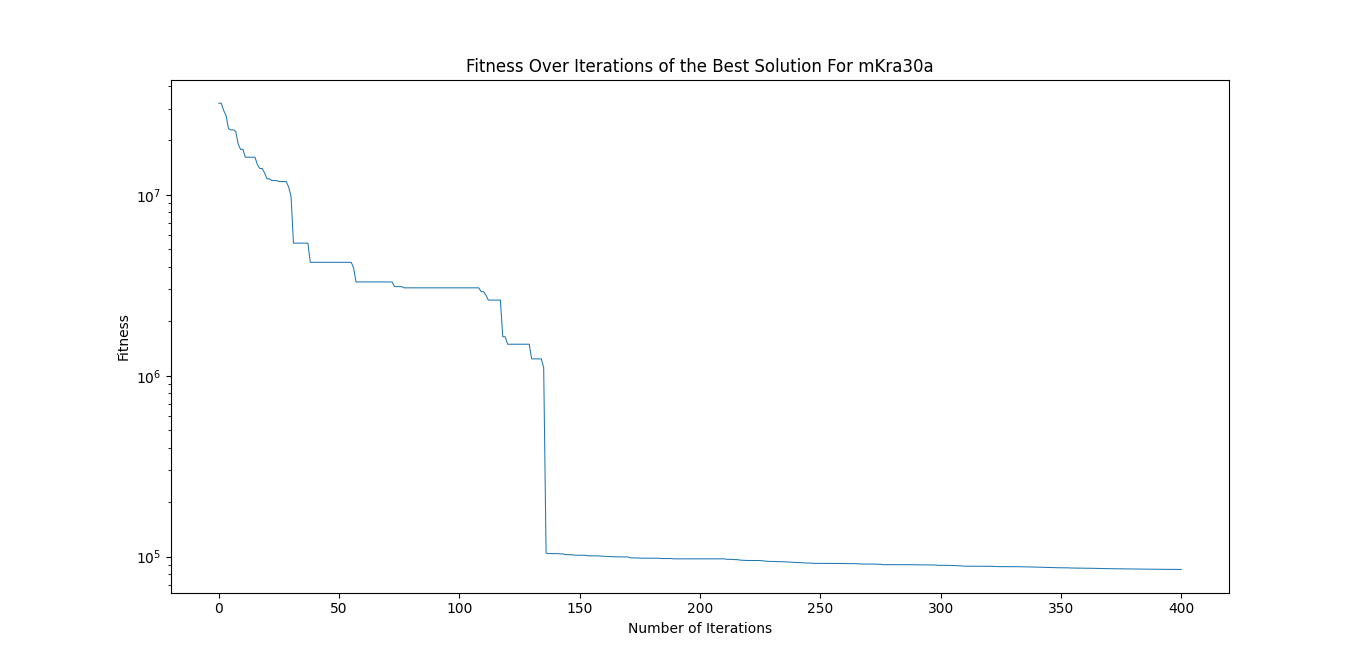
\includegraphics[scale=0.5]{./images/chap07-rd/gwo-only-mkra30a-best-solution-fitness-graph.png}
\end{adjustwidth}
\caption{The fitness of the best solution generated by $G_{50,8}$ as the number of iterations increasee while solving the mKra30a problem.}
\label{approach-gwo-mkra30a-best-solution-fitness-over-time}
\end{figure}

\begin{table}
\centering
\resizebox{0.5\textwidth}{!}{\rotatebox{90}{
\begin{tabular}{|r|r|r|r|r|r|r|} 
	\hline
	\multicolumn{2}{|c|}{\textbf{Parameters}}                                  & \multicolumn{5}{c|}{\textbf{SFLP-II}}                                                                                                                                                                     \\ 
	\hline
	\multicolumn{1}{|c|}{\textbf{Pop. Size}} & \multicolumn{1}{c|}{\textbf{c}} & \multicolumn{1}{c|}{\textbf{Best}} & \multicolumn{1}{c|}{\textbf{Worst}} & \multicolumn{1}{c|}{\textbf{Avg.}} & \multicolumn{1}{c|}{\textbf{Std. Dev.}} & \multicolumn{1}{c|}{\textbf{Avg. Runtime (s)}}  \\ 
	\hline
	\multirow{4}{*}{25}                      & 2                               & 226.149871                         & 328.546146                          & 287.749326366667                   & 24.7018482581174                        & 6.03333333333333                                \\ 
	\cline{2-7}
	& 4                               & 228.710226                         & 373.604858                          & 298.836421533333                   & 34.1522620177737                        & 5.9                                             \\ 
	\cline{2-7}
	& 8                               & 249.624192                         & 368.435807                          & 313.640670633333                   & 29.7958232730557                        & 6.23333333333333                                \\ 
	\cline{2-7}
	& 12                              & 255.639347                         & 358.033844                          & 315.207093933333                   & 26.4399229476443                        & 6.36666666666667                                \\ 
	\hline
	\multirow{4}{*}{50}                      & 2                               & 221.18019                          & 341.568304                          & 283.795019233333                   & 28.9742518867792                        & 13.2666666666667                                \\ 
	\cline{2-7}
	& 4                               & 241.862298                         & 389.711568                          & 294.2461242                        & 33.7641257773172                        & 13.1333333333333                                \\ 
	\cline{2-7}
	& 8                               & 240.638127                         & 413.077936                          & 299.553292466667                   & 40.469222577263                         & 12.7333333333333                                \\ 
	\cline{2-7}
	& 12                              & 261.869799                         & 381.586061                          & 315.831642166667                   & 31.7204847308938                        & 13.6666666666667                                \\ 
	\hline
	\multirow{4}{*}{75}                      & 2                               & 205.666955                         & 386.356476                          & 290.063388433333                   & 38.0436802516604                        & 18.8666666666667                                \\ 
	\cline{2-7}
	& 4                               & 239.258536                         & 406.790997                          & 302.005947566667                   & 39.1344289013742                        & 18.9                                            \\ 
	\cline{2-7}
	& 8                               & 246.916627                         & 393.744452                          & 309.957982766667                   & 32.0156308267039                        & 19.5                                            \\ 
	\cline{2-7}
	& 12                              & 243.386427                         & 413.874466                          & 307.3213231                        & 36.2239957721235                        & 19.3333333333333                                \\
	\hline
\end{tabular}}}
\caption{Summary of the experiments using the GWO approach with the SFLP-II problem.}
\label{full-data-gwo-sflp-ii}
\end{table}

\begin{table}
\centering
\resizebox{0.5\textwidth}{!}{\rotatebox{90}{
\begin{tabular}{|r|r|r|r|r|r|r|} 
	\hline
	\multicolumn{2}{|c|}{\textbf{Parameters}}                                  & \multicolumn{5}{c|}{\textbf{mSFLP-III}}                                                                                                                                                                   \\ 
	\hline
	\multicolumn{1}{|c|}{\textbf{Pop. Size}} & \multicolumn{1}{c|}{\textbf{c}} & \multicolumn{1}{c|}{\textbf{Best}} & \multicolumn{1}{c|}{\textbf{Worst}} & \multicolumn{1}{c|}{\textbf{Avg.}} & \multicolumn{1}{c|}{\textbf{Std. Dev.}} & \multicolumn{1}{c|}{\textbf{Avg. Runtime (s)}}  \\ 
	\hline
	\multirow{4}{*}{25}                      & 2                               & 50874.238564                       & 60974.998642                        & 55624.0061857667                   & 2544.70550235336                        & 22.4333333333333                                \\ 
	\cline{2-7}
	& 4                               & 50825.278824                       & 59194.486832                        & 55236.4286594                      & 2301.71070299619                        & 21.3333333333333                                \\ 
	\cline{2-7}
	& 8                               & 51250.638187                       & 57894.186882                        & 54206.6467008333                   & 1334.40810225102                        & 23.6                                            \\ 
	\cline{2-7}
	& 12                              & 51328.437737                       & 62758.004044                        & 55331.2312675333                   & 2540.54370041386                        & 21.2333333333333                                \\ 
	\hline
	\multirow{4}{*}{50}                      & 2                               & 47597.794662                       & 62827.738159                        & 54495.2676476667                   & 3328.18744058766                        & 40.1333333333333                                \\ 
	\cline{2-7}
	& 4                               & 50250.080536                       & 57916.673454                        & 53421.9267731333                   & 2239.06725435468                        & 41.9666666666667                                \\ 
	\cline{2-7}
	& 8                               & 48844.175789                       & 59710.615997                        & 52699.5983075667                   & 2062.76885562279                        & 41.2666666666667                                \\ 
	\cline{2-7}
	& 12                              & 48920.979538                       & 56477.689476                        & 52837.3591700333                   & 1980.22102755171                        & 42.2333333333333                                \\ 
	\hline
	\multirow{4}{*}{75}                      & 2                               & 50179.684898                       & 57659.66436                         & 54015.3749653                      & 2050.7167136713                         & 61.1                                            \\ 
	\cline{2-7}
	& 4                               & 48752.443314                       & 56156.624268                        & 52037.6629276                      & 2313.4004317195                         & 61.5333333333333                                \\ 
	\cline{2-7}
	& 8                               & 49276.248596                       & 54977.558044                        & 51801.8837937333                   & 1419.1918023338                         & 63.0333333333333                                \\ 
	\cline{2-7}
	& 12                              & 49644.232903                       & 55524.684891                        & 51837.8766529667                   & 1430.57988385005                        & 61.7666666666667                                \\
	\hline
\end{tabular}}}
\caption{Summary of the experiments using the GWO approach with the mSFLP-III problem.}
\label{full-data-gwo-msflp-iii}
\end{table}

\begin{table}
\centering
\resizebox{0.5\textwidth}{!}{\rotatebox{90}{
\begin{tabular}{|r|r|r|r|r|r|r|} 
	\hline
	\multicolumn{2}{|c|}{\textbf{Parameters}}                                  & \multicolumn{5}{c|}{\textbf{mKra30a}}                                                                                                                                                                     \\ 
	\hline
	\multicolumn{1}{|c|}{\textbf{Pop. Size}} & \multicolumn{1}{c|}{\textbf{c}} & \multicolumn{1}{l|}{\textbf{Best}} & \multicolumn{1}{l|}{\textbf{Worst}} & \multicolumn{1}{l|}{\textbf{Avg.}} & \multicolumn{1}{l|}{\textbf{Std. Dev.}} & \multicolumn{1}{l|}{\textbf{Avg. Runtime (s)}}  \\ 
	\hline
	\multirow{4}{*}{25}                      & 2                               & 94640.759514                       & 120397.403767                       & 107874.742523333                   & 6706.6049593287                         & 35.9666666666667                                \\ 
	\cline{2-7}
	& 4                               & 87110.57618                        & 116746.599121                       & 104270.487286567                   & 8041.05756072353                        & 36.3333333333333                                \\ 
	\cline{2-7}
	& 8                               & 95254.061554                       & 118719.490257                       & 105760.743434367                   & 6557.69877516131                        & 37.0666666666667                                \\ 
	\cline{2-7}
	& 12                              & 93525.765816                       & 124181.531029                       & 108251.9895637                     & 8151.19724950765                        & 37.3                                            \\ 
	\hline
	\multirow{4}{*}{50}                      & 2                               & 88657.824898                       & 121124.59779                        & 102742.1803823                     & 7156.18271087496                        & 73.3333333333333                                \\ 
	\cline{2-7}
	& 4                               & 90599.06601                        & 122300.269909                       & 102855.4831497                     & 8820.10238434929                        & 70.9666666666667                                \\ 
	\cline{2-7}
	& 8                               & 84929.672058                       & 112251.415863                       & 101570.163644533                   & 6490.61277032704                        & 72.1                                            \\ 
	\cline{2-7}
	& 12                              & 92563.720146                       & 128598.716599                       & 105348.4949903                     & 9267.72959691125                        & 69.5666666666667                                \\ 
	\hline
	\multirow{4}{*}{75}                      & 2                               & 88740.484344                       & 117173.305939                       & 99149.0616948                      & 5833.24082935413                        & 104.7                                           \\ 
	\cline{2-7}
	& 4                               & 89197.608078                       & 121878.61042                        & 99482.2352776                      & 7069.6968084522                         & 107.966666666667                                \\ 
	\cline{2-7}
	& 8                               & 87299.715054                       & 113760.078079                       & 98968.6223121                      & 6443.60722715266                        & 108.7                                           \\ 
	\cline{2-7}
	& 12                              & 86942.304199                       & 108422.175175                       & 98108.9092933667                   & 6511.43059062118                        & 111.266666666667                                \\
	\hline
\end{tabular}}}
\caption{Summary of the experiments using the GWO approach with the mKra30a problem.}
\label{full-data-gwo-mkra30a}
\end{table}

Each data set used in the experiments uses differently-sized bounding regions. For SFLP-II, a $12x12$ bounding region is used. mSFLP-III uses a $260x260$ bounding region, while mKra30a uses a $250x250$ one. Notice that, for the SFLP-II problem, configurations using $c = 2$ in each population size produce the best average fitness. For the mSFLP-III problems, regardless of population size, using $c = 8$ produces the best average fitness. This suggests to us that, for certain problems with at least less than 20 buildings, the ideal $c$ value to be used with our GWO approach have some correlation with the size of the bounding box. Smaller $c$ values are more likely to be better for problems with smaller bounding boxes. Similarly, larger $c$ values are more likely to better fit problems with larger bounding boxes. However, too high of a value for $c$ may produce worse results on average. This is shown to us by our results with the mSFLP-III problem, where, regardless of population size, configurations with $c = 8$ consistently perform better on average than those with $c = 12$. We can attribute this behaviour to the fact that the $c$ parameter determines how much a building can be shifted away in the formulas of $D_{\alpha}$, $D_{\beta}$, and $D_{\delta}$ (see equations \ref{summary-modified-gwo-a} to \ref{summary-modified-gwo-xt1} in Methodology). A smaller $c$ value introduces a smaller shift, while a larger value will shift the buildings further. In smaller sized bounding regions, a smaller shift is important due to the limited space available. Larger shifts in such a space will make it harder for buildings to reach feasibility. On the other hand, a larger shift is more appropriate in a larger space since it will allow buildings to move closer to each other faster. Moreover, such a larger amount of available space can be better utilized. A larger space will allow buildings to more easily move away from intersections (and, consequently, infeasibility). However, as shown by our experiments with the mSFLP-III problem, a configuration with the ability to shift too much (e.g. having a $c$ value of $12$) can perform poorer than one with a slightly lower amount of shifting. This is due to the fact that shifts that are too large can push and orient buildings in positions and orientations where, over time, it would become more difficult for them to move towards a position where they are close to other buildings as much as possible yet not intersecting with any of them. Buildings may actually move further away from or move in such a way that hinders them from progressing towards these better positions due to this amount of shifting, contributing to the difficulty. Other causes further exacerbate this behaviour. The gradual reduction of the amount of shifting buildings can do as time progresses (see Equation \ref{summary-modified-gwo-a}, which is the factor for this gradual reduction), makes it harder for buildings to shift towards a superior position and influencing them to only move within a gradually smaller local area. Another contributing factor to the behaviour is that buildings cluster together over time in our approach. This increases the risk of building intersections, especially those building that are nearer to the "inside" of a cluster.

Intriguingly, for the mKra30a problem (which has 30 buildings), the ideal $c$ value seems to have a correlation with the population size used. As the population size increases, the $c$ value must also be increased to be able to produce the best solutions possible. This is in contrary with the trend suggested by the experiments dealing with the first two problems. This may suggest that the parameters of a problem are also factors in determining the ideal value for $c$. However, additional experiments are needed to determine if this behaviour with the mKra30a problem is not a merely quirk caused by the random nature of metaheuristics. If ever it is found out to be an expected behaviour of our GWO approach when dealing with the mKra30a problem or a problem of similar or greater parameters, additional experiments should be able to provide insights as to why our approach has this behaviour.

It should also be mentioned that the average runtime of each experiment setup in each population size category are generally almost equal to each other. However, the experiments dealing with the mKra30a problem with population sizes of $50$ and $75$ have larger deviations from each other. It is of interesting note that for the experiment configurations with a population size of $75$ solving the mKra30a problem, the average runtime increases as the $c$ value increases.

We also observe that the population size has an impact on the performance of our GWO approach. For larger-sized problems with large bounding boxes such as mSFLP-III and mKra30a, our experiments show that, on average, a larger population size is more ideal. We argue that this is due to the larger amount of space the wolves/solutions cover in the abstract search space, which becomes larger as the size of the problem increases. A diverse set of initial solutions resulting from the larger population size allows for this larger amount of covered space. This naturally allows us to more easily find the best possible solution for a problem within a reasonable amount of time compared to with a smaller population size. On the contrary and quite interestingly, for small-sized problems with smaller-sized bounding boxes, such as SFLP-II, our experiments show that the higher population sizes do not necessarily translate to better solutions on average. It is suggested by our experiments that a medium-sized population with the right $c$ value produces the best possible solutions for these small-sized problems compared to using the other two population sizes, with small-sized populations performing surprisingly better than large-sized ones, again with both using the best $c$ value for the population size. This is rather odd given the advantage of having a larger population. It would make sense for experiments with medium-sized populations and the right $c$ value to perform than their small-sized population counterparts. However, it does not immediately make sense why the large-sized population experiments would perform poorly than the small-sized ones. In any case, they should perform better, especially when against the medium-sized population. A possible explanation to this is that a larger population size for small-sized problems may result in achieving local optimum too fast. As per the behaviour of GWO itself, wolves/solutions would gradually cluster around this local optimum until a new better local optimum is found to cluster towards to. We argue that finding another local optimum would be more difficult, since SFLP-II has smaller bounding region size. Intersections between buildings will occur more frequently compared to when using a larger bounding region. Hence, our approach finds it harder to find a better local optimum, resulting in worse average results. Further studies would be needed to gain a better understanding of this behaviour, to confirm our hypothesis, and to determine whether this is simply a quirk of randomness or not.

Later research may also want to focus on determining the ideal $c$ value and population size for a certain problem based on the problem parameters. Figuring out whether the $c$ value can be mathematically modelled rather than being a parameter is another possible avenue for research.

% Start of the GWO table of results for the one with a population of 25.
\begin{table}
\centering
\begin{adjustwidth}{}{}
\resizebox{\textwidth}{!}{\rotatebox{90}{
\begin{tabular}{|r|r|r|r|r|r|r|}
\hline
\multicolumn{1}{|c|}{\multirow{2}{*}{Run}} & \multicolumn{6}{c|}{GWO (c = 2, Pop. Size of 25)}                                                                                                                                                                                      \\ 
\cline{2-7}
\multicolumn{1}{|c|}{}                     & \multicolumn{1}{l|}{SFLP-II} & \multicolumn{1}{l|}{Elapsed Time (s)} & \multicolumn{1}{l|}{mSFLP-III} & \multicolumn{1}{l|}{Elapsed Time (s)} & \multicolumn{1}{l|}{mKra30a} & \multicolumn{1}{l|}{Elapsed Time (s)}  \\ 
\hline
1                                          & 284.274332                   & 5                                     & 54517.212997                   & 20                                    & 113444.272751                & 34                                     \\ 
\hline
2                                          & 279.224484                   & 6                                     & 55100.110451                   & 25                                    & 108634.12896                 & 35                                     \\ 
\hline
3                                          & 290.766824                   & 7                                     & 54424.891159                   & 20                                    & 101057.257011                & 36                                     \\ 
\hline
4                                          & 255.89164                    & 6                                     & 52281.025963                   & 21                                    & 106933.341133                & 36                                     \\ 
\hline
5                                          & 303.41135                    & 6                                     & 56333.281975                   & 24                                    & 110198.061668                & 37                                     \\ 
\hline
6                                          & 307.247426                   & 6                                     & 56191.257446                   & 23                                    & 103150.565979                & 35                                     \\ 
\hline
7                                          & 297.32725                    & 6                                     & 57228.114368                   & 26                                    & 100159.379417                & 34                                     \\ 
\hline
8                                          & 298.901143                   & 6                                     & 54501.928665                   & 25                                    & 94640.759514                 & 36                                     \\ 
\hline
9                                          & 290.924892                   & 6                                     & 60974.998642                   & 22                                    & 101369.649643                & 35                                     \\ 
\hline
10                                         & 328.546146                   & 5                                     & 52108.460861                   & 23                                    & 114400.855766                & 34                                     \\ 
\hline
11                                         & 310.501635                   & 6                                     & 55957.510098                   & 21                                    & 108862.321945                & 39                                     \\ 
\hline
12                                         & 260.87289                    & 5                                     & 55527.02594                    & 24                                    & 106595.717178                & 39                                     \\ 
\hline
13                                         & 282.531157                   & 5                                     & 58757.132118                   & 20                                    & 115065.923737                & 34                                     \\ 
\hline
14                                         & 260.606181                   & 7                                     & 60825.496319                   & 22                                    & 109135.383606                & 35                                     \\ 
\hline
15                                         & 315.86567                    & 6                                     & 52600.283459                   & 20                                    & 120397.403767                & 35                                     \\ 
\hline
16                                         & 277.906986                   & 7                                     & 59222.901581                   & 24                                    & 114673.857002                & 39                                     \\ 
\hline
17                                         & 313.385026                   & 6                                     & 53981.477821                   & 24                                    & 96989.450607                 & 36                                     \\ 
\hline
18                                         & 289.163818                   & 6                                     & 57612.964134                   & 23                                    & 104600.307762                & 37                                     \\ 
\hline
19                                         & 275.85824                    & 5                                     & 58171.204727                   & 20                                    & 104245.289139                & 36                                     \\ 
\hline
20                                         & 317.423512                   & 7                                     & 57049.199783                   & 20                                    & 114823.94133                 & 36                                     \\ 
\hline
21                                         & 288.800416                   & 6                                     & 52996.785149                   & 23                                    & 108857.258942                & 34                                     \\ 
\hline
22                                         & 311.202401                   & 6                                     & 54449.246704                   & 23                                    & 102069.259422                & 36                                     \\ 
\hline
23                                         & 226.149871                   & 7                                     & 53806.471344                   & 21                                    & 95024.52264                  & 35                                     \\ 
\hline
24                                         & 258.801216                   & 5                                     & 58588.215469                   & 22                                    & 113719.784393                & 36                                     \\ 
\hline
25                                         & 268.787345                   & 7                                     & 53098.863617                   & 22                                    & 105550.2397                  & 36                                     \\ 
\hline
26                                         & 290.496099                   & 6                                     & 50874.238564                   & 21                                    & 108321.213905                & 35                                     \\ 
\hline
27                                         & 318.591564                   & 7                                     & 54556.366089                   & 25                                    & 110759.756439                & 35                                     \\ 
\hline
28                                         & 253.100093                   & 6                                     & 55594.022305                   & 22                                    & 119703.695831                & 37                                     \\ 
\hline
29                                         & 257.999482                   & 6                                     & 54408.740974                   & 25                                    & 108653.213264                & 39                                     \\ 
\hline
30                                         & 317.920702                   & 6                                     & 56980.756851                   & 22                                    & 114205.463249                & 38                                     \\ 
\hline
\multicolumn{1}{|l|}{Average}              & 287.749326366667             & 6.03333333333333                      & 55624.0061857667               & 22.4333333333333                      & 107874.742523333             & 35.9666666666667                       \\ 
\hline
\multicolumn{1}{|l|}{Std. Dev}             & 24.7018482581174             & 0.668675135459372                     & 2544.70550235336               & 1.81342376380328                      & 6706.6049593287              & 1.56432938883779                       \\
\hline
\end{tabular}}}
\end{adjustwidth}
\caption{The entire experiment data we have collected using our GWO approach with $c = 2$ and a population of $25$.}
\label{full-data-gwo-c2-p25}
\end{table}

\begin{table}
\centering
\begin{adjustwidth}{}{}
\resizebox{\textwidth}{!}{\rotatebox{90}{
\begin{tabular}{|r|r|r|r|r|r|r|}
\hline
\multicolumn{1}{|c|}{\multirow{2}{*}{Run}} & \multicolumn{6}{c|}{GWO (c = 4, Pop. Size of 25)}                                                                                                                                                                     \\ 
\cline{2-7}
\multicolumn{1}{|c|}{}                     & \multicolumn{1}{l|}{SFLP-II} & \multicolumn{1}{l|}{Elapsed Time (s)} & \multicolumn{1}{l|}{mSFLP-III} & \multicolumn{1}{l|}{Elapsed Time (s)} & \multicolumn{1}{l|}{mKra30a} & \multicolumn{1}{l|}{Elapsed Time (s)}  \\ 
\hline
1                                          & 295.290119                   & 5                                     & 57590.204044                   & 21                                    & 99250.338013                 & 36                                     \\ 
\hline
2                                          & 364.30381                    & 6                                     & 55786.4907                     & 19                                    & 115392.5942                  & 36                                     \\ 
\hline
3                                          & 283.958384                   & 6                                     & 56478.70369                    & 19                                    & 100622.106056                & 34                                     \\ 
\hline
4                                          & 308.185705                   & 6                                     & 59149.522892                   & 21                                    & 100370.279572                & 37                                     \\ 
\hline
5                                          & 279.100698                   & 5                                     & 52092.835846                   & 24                                    & 109341.424805                & 40                                     \\ 
\hline
6                                          & 254.694568                   & 7                                     & 54517.030029                   & 23                                    & 111078.602165                & 34                                     \\ 
\hline
7                                          & 299.122021                   & 5                                     & 57337.25061                    & 25                                    & 87110.57618                  & 38                                     \\ 
\hline
8                                          & 308.245055                   & 5                                     & 56083.913353                   & 21                                    & 116746.599121                & 36                                     \\ 
\hline
9                                          & 310.631233                   & 6                                     & 56986.768219                   & 19                                    & 112465.605843                & 37                                     \\ 
\hline
10                                         & 293.218722                   & 6                                     & 53868.101875                   & 21                                    & 110742.670616                & 37                                     \\ 
\hline
11                                         & 290.615551                   & 7                                     & 55411.816826                   & 21                                    & 102156.222603                & 39                                     \\ 
\hline
12                                         & 310.314302                   & 6                                     & 50825.278824                   & 24                                    & 112943.161697                & 34                                     \\ 
\hline
13                                         & 284.625909                   & 6                                     & 51448.845734                   & 21                                    & 96147.747742                 & 34                                     \\ 
\hline
14                                         & 330.488841                   & 6                                     & 57670.047066                   & 22                                    & 106707.319443                & 37                                     \\ 
\hline
15                                         & 271.799747                   & 6                                     & 57224.530266                   & 21                                    & 106312.161995                & 41                                     \\ 
\hline
16                                         & 308.069251                   & 7                                     & 53504.969574                   & 21                                    & 109508.693184                & 39                                     \\ 
\hline
17                                         & 307.75226                    & 6                                     & 54594.552979                   & 22                                    & 98866.16114                  & 34                                     \\ 
\hline
18                                         & 241.580049                   & 6                                     & 56112.939285                   & 19                                    & 103499.234871                & 33                                     \\ 
\hline
19                                         & 228.710226                   & 6                                     & 56761.539284                   & 23                                    & 88510.688866                 & 35                                     \\ 
\hline
20                                         & 291.547085                   & 6                                     & 56455.574303                   & 22                                    & 97130.734337                 & 38                                     \\ 
\hline
21                                         & 373.604858                   & 5                                     & 59194.486832                   & 23                                    & 115666.25502                 & 32                                     \\ 
\hline
22                                         & 288.904785                   & 7                                     & 51962.636154                   & 20                                    & 100993.999092                & 37                                     \\ 
\hline
23                                         & 351.234066                   & 5                                     & 54615.561333                   & 20                                    & 108507.541492                & 35                                     \\ 
\hline
24                                         & 271.269831                   & 6                                     & 52326.159271                   & 20                                    & 102196.612885                & 35                                     \\ 
\hline
25                                         & 345.786381                   & 7                                     & 55869.035088                   & 21                                    & 106251.775101                & 40                                     \\ 
\hline
26                                         & 251.753436                   & 6                                     & 53282.332359                   & 20                                    & 94795.74794                  & 36                                     \\ 
\hline
27                                         & 316.554537                   & 5                                     & 53018.602661                   & 22                                    & 110122.478073                & 36                                     \\ 
\hline
28                                         & 321.758455                   & 5                                     & 58369.596535                   & 20                                    & 94860.329987                 & 42                                     \\ 
\hline
29                                         & 263.652587                   & 6                                     & 55446.598206                   & 21                                    & 95583.080429                 & 33                                     \\ 
\hline
30                                         & 318.320174                   & 6                                     & 53106.935944                   & 24                                    & 114233.876129                & 35                                     \\ 
\hline
\multicolumn{1}{|l|}{Average}              & 298.836421533333             & 5.9                                   & 55236.4286594                  & 21.3333333333333                      & 104270.487286567             & 36.3333333333333                       \\ 
\hline
\multicolumn{1}{|l|}{Std. Dev}             & 34.1522620177737             & 0.661763578993857                     & 2301.71070299619               & 1.62593916273628                      & 8041.05756072353             & 2.48211996894386                       \\
\hline
\end{tabular}}}
\end{adjustwidth}
\caption{The entire experiment data we have collected using our GWO approach with $c = 4$ and a population of $25$.}
\label{full-data-gwo-c4-p25}
\end{table}

\begin{table}
\centering
\begin{adjustwidth}{}{}
\resizebox{\textwidth}{!}{\rotatebox{90}{
\begin{tabular}{|r|r|r|r|r|r|r|}
\hline
\multicolumn{1}{|c|}{\multirow{2}{*}{Run}} & \multicolumn{6}{c|}{GWO (c = 8, Pop. Size of 25)}                                                                                                                                                                     \\ 
\cline{2-7}
\multicolumn{1}{|c|}{}                     & \multicolumn{1}{l|}{SFLP-II} & \multicolumn{1}{l|}{Elapsed Time (s)} & \multicolumn{1}{l|}{mSFLP-III} & \multicolumn{1}{l|}{Elapsed Time (s)} & \multicolumn{1}{l|}{mKra30a} & \multicolumn{1}{l|}{Elapsed Time (s)}  \\ 
\hline
1                                          & 262.707255                   & 7                                     & 55466.377586                   & 20                                    & 104697.724777                & 37                                     \\ 
\hline
2                                          & 311.009165                   & 6                                     & 52879.782005                   & 20                                    & 114784.794098                & 41                                     \\ 
\hline
3                                          & 291.360188                   & 6                                     & 54291.537682                   & 22                                    & 106627.593742                & 34                                     \\ 
\hline
4                                          & 362.348913                   & 5                                     & 51966.878838                   & 22                                    & 118225.260605                & 36                                     \\ 
\hline
5                                          & 305.725908                   & 7                                     & 57894.186882                   & 22                                    & 107491.358063                & 37                                     \\ 
\hline
6                                          & 344.391756                   & 5                                     & 54056.77681                    & 24                                    & 118719.490257                & 36                                     \\ 
\hline
7                                          & 337.822041                   & 6                                     & 53829.962364                   & 24                                    & 100109.010674                & 33                                     \\ 
\hline
8                                          & 319.080408                   & 7                                     & 53949.482574                   & 23                                    & 96509.502808                 & 38                                     \\ 
\hline
9                                          & 249.624192                   & 7                                     & 55062.295784                   & 22                                    & 95254.061554                 & 38                                     \\ 
\hline
10                                         & 317.502579                   & 8                                     & 54612.372421                   & 22                                    & 111357.790108                & 34                                     \\ 
\hline
11                                         & 347.870933                   & 6                                     & 55273.090096                   & 25                                    & 99750.327438                 & 37                                     \\ 
\hline
12                                         & 294.693992                   & 7                                     & 54738.413105                   & 25                                    & 106767.40667                 & 35                                     \\ 
\hline
13                                         & 282.647407                   & 7                                     & 54133.133018                   & 25                                    & 111462.286797                & 34                                     \\ 
\hline
14                                         & 292.732835                   & 6                                     & 54017.253056                   & 24                                    & 107217.431229                & 39                                     \\ 
\hline
15                                         & 283.872915                   & 5                                     & 53602.699944                   & 26                                    & 106198.506428                & 44                                     \\ 
\hline
16                                         & 321.749494                   & 7                                     & 54680.752884                   & 23                                    & 97637.581284                 & 36                                     \\ 
\hline
17                                         & 310.098661                   & 5                                     & 53654.185509                   & 23                                    & 97815.004234                 & 34                                     \\ 
\hline
18                                         & 292.552563                   & 5                                     & 54514.880905                   & 26                                    & 104283.744904                & 39                                     \\ 
\hline
19                                         & 330.776446                   & 6                                     & 54886.626793                   & 23                                    & 108294.5578                  & 47                                     \\ 
\hline
20                                         & 368.435807                   & 5                                     & 51250.638187                   & 25                                    & 101209.694763                & 35                                     \\ 
\hline
21                                         & 333.208825                   & 5                                     & 53291.312008                   & 22                                    & 104063.487877                & 39                                     \\ 
\hline
22                                         & 307.813316                   & 6                                     & 54018.854462                   & 26                                    & 106063.043762                & 34                                     \\ 
\hline
23                                         & 326.428337                   & 6                                     & 55304.592007                   & 26                                    & 99203.966431                 & 37                                     \\ 
\hline
24                                         & 358.536934                   & 5                                     & 56567.198547                   & 25                                    & 114660.357567                & 36                                     \\ 
\hline
25                                         & 299.608566                   & 6                                     & 52027.762772                   & 26                                    & 101201.104996                & 38                                     \\ 
\hline
26                                         & 288.695351                   & 8                                     & 55043.384789                   & 23                                    & 100895.692963                & 38                                     \\ 
\hline
27                                         & 320.946527                   & 7                                     & 54383.856281                   & 22                                    & 110844.852486                & 40                                     \\ 
\hline
28                                         & 363.365827                   & 9                                     & 53825.792953                   & 23                                    & 104716.713264                & 33                                     \\ 
\hline
29                                         & 289.365061                   & 6                                     & 54623.883316                   & 25                                    & 100086.231628                & 35                                     \\ 
\hline
30                                         & 294.247917                   & 6                                     & 52351.437447                   & 24                                    & 116673.723824                & 38                                     \\ 
\hline
\multicolumn{1}{|l|}{Average}              & 313.640670633333             & 6.23333333333333                      & 54206.6467008333               & 23.6                                  & 105760.743434367             & 37.0666666666667                       \\ 
\hline
\multicolumn{1}{|l|}{Std. Dev}             & 29.7958232730557             & 1.04000442085709                      & 1334.40810225102               & 1.7340405277052                       & 6557.69877516131             & 3.12865877767558                       \\
\hline
\end{tabular}}}
\end{adjustwidth}
\caption{The entire experiment data we have collected using our GWO approach with $c = 8$ and a population of $25$.}
\label{full-data-gwo-c8-p25}
\end{table}

\begin{table}
\centering
\begin{adjustwidth}{}{}
\resizebox{\textwidth}{!}{\rotatebox{90}{
\begin{tabular}{|r|r|r|r|r|r|r|}
\hline
\multicolumn{1}{|c|}{\multirow{2}{*}{Run}} & \multicolumn{6}{c|}{GWO (c = 12, Pop. Size of 25)}                                                                                                                                                                    \\ 
\cline{2-7}
\multicolumn{1}{|c|}{}                     & \multicolumn{1}{l|}{SFLP-II} & \multicolumn{1}{l|}{Elapsed Time (s)} & \multicolumn{1}{l|}{mSFLP-III} & \multicolumn{1}{l|}{Elapsed Time (s)} & \multicolumn{1}{l|}{mKra30a} & \multicolumn{1}{l|}{Elapsed Time (s)}  \\ 
\hline
1                                          & 280.100084                   & 6                                     & 54382.193893                   & 22                                    & 110420.231773                & 35                                     \\ 
\hline
2                                          & 326.000024                   & 6                                     & 56657.682411                   & 19                                    & 107836.336555                & 39                                     \\ 
\hline
3                                          & 339.59429                    & 6                                     & 56128.932846                   & 20                                    & 105101.680847                & 34                                     \\ 
\hline
4                                          & 291.153993                   & 6                                     & 56149.892471                   & 22                                    & 99260.377151                 & 36                                     \\ 
\hline
5                                          & 324.951407                   & 6                                     & 57060.862228                   & 22                                    & 97755.446457                 & 39                                     \\ 
\hline
6                                          & 322.430838                   & 6                                     & 62758.004044                   & 20                                    & 114021.624924                & 38                                     \\ 
\hline
7                                          & 325.058099                   & 6                                     & 54246.820145                   & 20                                    & 100348.282265                & 36                                     \\ 
\hline
8                                          & 301.274588                   & 6                                     & 54187.122147                   & 20                                    & 97531.603271                 & 40                                     \\ 
\hline
9                                          & 341.434416                   & 8                                     & 53573.432259                   & 19                                    & 108106.979767                & 37                                     \\ 
\hline
10                                         & 357.480109                   & 7                                     & 56897.296356                   & 23                                    & 116657.657318                & 37                                     \\ 
\hline
11                                         & 345.915623                   & 7                                     & 51811.845238                   & 21                                    & 109709.232689                & 33                                     \\ 
\hline
12                                         & 321.136856                   & 6                                     & 53061.549057                   & 24                                    & 100745.31324                 & 40                                     \\ 
\hline
13                                         & 327.757973                   & 6                                     & 52248.577141                   & 24                                    & 107016.641022                & 36                                     \\ 
\hline
14                                         & 338.574615                   & 7                                     & 55548.896332                   & 26                                    & 105929.138687                & 39                                     \\ 
\hline
15                                         & 354.648388                   & 6                                     & 53266.573128                   & 23                                    & 110405.852989                & 36                                     \\ 
\hline
16                                         & 305.538115                   & 7                                     & 54944.865646                   & 22                                    & 121917.463058                & 36                                     \\ 
\hline
17                                         & 274.450367                   & 6                                     & 52603.816597                   & 20                                    & 118235.825241                & 37                                     \\ 
\hline
18                                         & 299.440072                   & 7                                     & 54888.153915                   & 22                                    & 116887.253868                & 36                                     \\ 
\hline
19                                         & 320.987788                   & 8                                     & 56474.669212                   & 20                                    & 102034.555359                & 37                                     \\ 
\hline
20                                         & 317.335714                   & 7                                     & 59091.504066                   & 18                                    & 93525.765816                 & 38                                     \\ 
\hline
21                                         & 358.033844                   & 5                                     & 53225.246391                   & 20                                    & 105195.959213                & 37                                     \\ 
\hline
22                                         & 296.381484                   & 6                                     & 56367.015659                   & 22                                    & 107206.72065                 & 39                                     \\ 
\hline
23                                         & 340.041138                   & 6                                     & 55241.328114                   & 21                                    & 122687.700439                & 39                                     \\ 
\hline
24                                         & 307.116007                   & 7                                     & 54713.23642                    & 20                                    & 105925.402702                & 37                                     \\ 
\hline
25                                         & 255.639347                   & 7                                     & 58269.998817                   & 20                                    & 124181.531029                & 35                                     \\ 
\hline
26                                         & 296.414082                   & 5                                     & 56489.390518                   & 18                                    & 99701.346191                 & 36                                     \\ 
\hline
27                                         & 264.475464                   & 6                                     & 51328.437737                   & 22                                    & 98267.529518                 & 40                                     \\ 
\hline
28                                         & 304.718431                   & 6                                     & 60483.979401                   & 26                                    & 116802.36039                 & 36                                     \\ 
\hline
29                                         & 305.344853                   & 6                                     & 53979.122162                   & 20                                    & 112001.866364                & 38                                     \\ 
\hline
30                                         & 312.784809                   & 7                                     & 53856.493675                   & 21                                    & 112142.008118                & 43                                     \\ 
\hline
\multicolumn{1}{|l|}{Average}              & 315.207093933333             & 6.36666666666667                      & 55331.2312675333               & 21.2333333333333                      & 108251.9895637               & 37.3                                   \\ 
\hline
\multicolumn{1}{|l|}{Std. Dev}             & 26.4399229476443             & 0.718395402284138                     & 2540.54370041386               & 2.01174711054387                      & 8151.19724950765             & 2.07031565142896                       \\
\hline
\end{tabular}}}
\end{adjustwidth}
\caption{The entire experiment data we have collected using our GWO approach with $c = 12$ and a population of $25$.}
\label{full-data-gwo-c12-p25}
\end{table}

% Start of the GWO table of results for the one with a population of 50.
\begin{table}
	\centering
	\begin{adjustwidth}{}{}
		\resizebox{\textwidth}{!}{\rotatebox{90}{
				\begin{tabular}{|r|r|r|r|r|r|r|}
					\hline
					\multicolumn{1}{|c|}{\multirow{2}{*}{Run}} & \multicolumn{6}{c|}{GWO (c = 2, Pop. 50)}                                                                                                                                                                             \\ 
					\cline{2-7}
					\multicolumn{1}{|c|}{}                     & \multicolumn{1}{l|}{SFLP-II} & \multicolumn{1}{l|}{Elapsed Time (s)} & \multicolumn{1}{l|}{mSFLP-III} & \multicolumn{1}{l|}{Elapsed Time (s)} & \multicolumn{1}{l|}{mKra30a} & \multicolumn{1}{l|}{Elapsed Time (s)}  \\ 
					\hline
					1                                          & 252.959127                   & 13                                    & 54847.391106                   & 39                                    & 115453.917747                & 71                                     \\ 
					\hline
					2                                          & 310.451593                   & 13                                    & 53073.76783                    & 40                                    & 105585.975105                & 71                                     \\ 
					\hline
					3                                          & 324.7657                     & 14                                    & 52564.010193                   & 39                                    & 96569.906059                 & 73                                     \\ 
					\hline
					4                                          & 302.253564                   & 12                                    & 62827.738159                   & 42                                    & 88657.824898                 & 69                                     \\ 
					\hline
					5                                          & 287.59426                    & 15                                    & 50270.968304                   & 38                                    & 99648.274292                 & 72                                     \\ 
					\hline
					6                                          & 246.890955                   & 12                                    & 51021.870609                   & 39                                    & 121124.59779                 & 68                                     \\ 
					\hline
					7                                          & 329.037109                   & 11                                    & 53698.933483                   & 39                                    & 109386.855927                & 74                                     \\ 
					\hline
					8                                          & 270.753061                   & 12                                    & 48938.991478                   & 37                                    & 100284.722839                & 68                                     \\ 
					\hline
					9                                          & 297.364378                   & 14                                    & 51457.838638                   & 39                                    & 102671.318954                & 72                                     \\ 
					\hline
					10                                         & 297.396819                   & 14                                    & 55029.144333                   & 40                                    & 100138.233009                & 72                                     \\ 
					\hline
					11                                         & 264.955059                   & 13                                    & 54034.453362                   & 44                                    & 94063.746262                 & 78                                     \\ 
					\hline
					12                                         & 239.019053                   & 13                                    & 54843.412094                   & 39                                    & 107732.370728                & 76                                     \\ 
					\hline
					13                                         & 269.378189                   & 15                                    & 60974.241631                   & 40                                    & 100197.140274                & 78                                     \\ 
					\hline
					14                                         & 270.275415                   & 13                                    & 53123.451248                   & 41                                    & 112261.793114                & 75                                     \\ 
					\hline
					15                                         & 245.398331                   & 13                                    & 56983.71854                    & 42                                    & 112999.618805                & 72                                     \\ 
					\hline
					16                                         & 288.427367                   & 13                                    & 55207.566151                   & 43                                    & 105895.490013                & 74                                     \\ 
					\hline
					17                                         & 233.585352                   & 13                                    & 57260.047424                   & 39                                    & 98834.100918                 & 75                                     \\ 
					\hline
					18                                         & 280.347926                   & 16                                    & 58842.573586                   & 39                                    & 101081.708069                & 76                                     \\ 
					\hline
					19                                         & 307.761939                   & 14                                    & 52738.607117                   & 39                                    & 99121.191231                 & 73                                     \\ 
					\hline
					20                                         & 284.018757                   & 13                                    & 53894.438091                   & 42                                    & 99270.817657                 & 75                                     \\ 
					\hline
					21                                         & 280.025665                   & 14                                    & 53150.059753                   & 39                                    & 113995.070282                & 72                                     \\ 
					\hline
					22                                         & 281.777046                   & 13                                    & 47597.794662                   & 42                                    & 99077.873138                 & 73                                     \\ 
					\hline
					23                                         & 221.18019                    & 14                                    & 53971.207901                   & 39                                    & 103581.175766                & 81                                     \\ 
					\hline
					24                                         & 308.542643                   & 14                                    & 53825.842094                   & 38                                    & 100780.563087                & 69                                     \\ 
					\hline
					25                                         & 302.184198                   & 13                                    & 59349.959862                   & 40                                    & 94936.180672                 & 73                                     \\ 
					\hline
					26                                         & 293.481107                   & 12                                    & 56370.238155                   & 43                                    & 97659.466835                 & 69                                     \\ 
					\hline
					27                                         & 300.88667                    & 13                                    & 51595.317627                   & 43                                    & 93650.395554                 & 76                                     \\ 
					\hline
					28                                         & 308.646566                   & 13                                    & 57071.090172                   & 37                                    & 103402.549973                & 74                                     \\ 
					\hline
					29                                         & 272.924234                   & 13                                    & 55864.520546                   & 41                                    & 103434.275482                & 77                                     \\ 
					\hline
					30                                         & 341.568304                   & 13                                    & 54428.835281                   & 42                                    & 100768.256989                & 74                                     \\ 
					\hline
					\multicolumn{1}{|l|}{Average}              & 283.795019233333             & 13.2666666666667                      & 54495.2676476667               & 40.1333333333333                      & 102742.1803823               & 73.3333333333333                       \\ 
					\hline
					\multicolumn{1}{|l|}{Std. Dev}             & 28.9742518867792             & 1.01483252680985                      & 3328.18744058766               & 1.87052147133163                      & 7156.18271087496             & 3.110974271758                         \\
					\hline
		\end{tabular}}}
	\end{adjustwidth}
	\caption{The entire experiment data we have collected using our GWO approach with $c = 2$ and a population of $50$.}
	\label{full-data-gwo-c2-p50}
\end{table}

\begin{table}
	\centering
	\begin{adjustwidth}{}{}
		\resizebox{\textwidth}{!}{\rotatebox{90}{
				\begin{tabular}{|r|r|r|r|r|r|r|}
					\hline
					\multicolumn{1}{|c|}{\multirow{2}{*}{Run}} & \multicolumn{6}{c|}{GWO (c = 4, Pop. 50)}                                                                                                                                                                             \\ 
					\cline{2-7}
					\multicolumn{1}{|c|}{}                     & \multicolumn{1}{l|}{SFLP-II} & \multicolumn{1}{l|}{Elapsed Time (s)} & \multicolumn{1}{l|}{mSFLP-III} & \multicolumn{1}{l|}{Elapsed Time (s)} & \multicolumn{1}{l|}{mKra30a} & \multicolumn{1}{l|}{Elapsed Time (s)}  \\ 
					\hline
					1                                          & 312.340316                   & 12                                    & 53062.125809                   & 43                                    & 91596.268288                 & 75                                     \\ 
					\hline
					2                                          & 292.071671                   & 14                                    & 51271.728905                   & 41                                    & 118655.595436                & 74                                     \\ 
					\hline
					3                                          & 329.653256                   & 12                                    & 55060.696541                   & 41                                    & 102449.075523                & 72                                     \\ 
					\hline
					4                                          & 306.763128                   & 16                                    & 57916.673454                   & 43                                    & 104931.357796                & 71                                     \\ 
					\hline
					5                                          & 252.772092                   & 12                                    & 50881.148052                   & 45                                    & 122300.269909                & 79                                     \\ 
					\hline
					6                                          & 351.977179                   & 14                                    & 53539.74173                    & 42                                    & 93781.166649                 & 67                                     \\ 
					\hline
					7                                          & 330.62476                    & 15                                    & 54803.86525                    & 38                                    & 108907.169487                & 71                                     \\ 
					\hline
					8                                          & 389.711568                   & 11                                    & 55295.007942                   & 39                                    & 95312.145584                 & 68                                     \\ 
					\hline
					9                                          & 297.27606                    & 13                                    & 53283.531433                   & 38                                    & 90647.4767                   & 67                                     \\ 
					\hline
					10                                         & 277.617715                   & 14                                    & 54563.107239                   & 40                                    & 93732.829643                 & 78                                     \\ 
					\hline
					11                                         & 266.562111                   & 12                                    & 52247.270363                   & 43                                    & 109087.634438                & 72                                     \\ 
					\hline
					12                                         & 300.58802                    & 13                                    & 53049.529968                   & 43                                    & 95105.831413                 & 71                                     \\ 
					\hline
					13                                         & 263.685979                   & 14                                    & 56017.20726                    & 44                                    & 110646.846546                & 69                                     \\ 
					\hline
					14                                         & 301.834932                   & 12                                    & 50960.144783                   & 37                                    & 101672.54467                 & 72                                     \\ 
					\hline
					15                                         & 295.790956                   & 15                                    & 54146.704651                   & 38                                    & 116249.322273                & 74                                     \\ 
					\hline
					16                                         & 268.800616                   & 13                                    & 50250.080536                   & 42                                    & 90599.06601                  & 70                                     \\ 
					\hline
					17                                         & 287.1534                     & 12                                    & 51163.562675                   & 39                                    & 112135.693672                & 69                                     \\ 
					\hline
					18                                         & 294.190074                   & 12                                    & 56055.587646                   & 40                                    & 102759.575096                & 70                                     \\ 
					\hline
					19                                         & 257.069981                   & 12                                    & 52603.173042                   & 43                                    & 99055.68399                  & 76                                     \\ 
					\hline
					20                                         & 247.273698                   & 13                                    & 54079.614361                   & 38                                    & 106487.916885                & 73                                     \\ 
					\hline
					21                                         & 241.862298                   & 13                                    & 54716.540192                   & 44                                    & 114099.514786                & 70                                     \\ 
					\hline
					22                                         & 314.056355                   & 12                                    & 51900.551003                   & 46                                    & 101358.406052                & 68                                     \\ 
					\hline
					23                                         & 304.7226                     & 14                                    & 50370.735947                   & 43                                    & 91041.143768                 & 69                                     \\ 
					\hline
					24                                         & 325.064058                   & 12                                    & 51801.091309                   & 45                                    & 95614.268036                 & 67                                     \\ 
					\hline
					25                                         & 298.000466                   & 13                                    & 56852.344414                   & 46                                    & 102250.452179                & 70                                     \\ 
					\hline
					26                                         & 243.562194                   & 15                                    & 54890.816574                   & 45                                    & 111223.215179                & 70                                     \\ 
					\hline
					27                                         & 275.810019                   & 12                                    & 57815.042976                   & 45                                    & 104611.12146                 & 71                                     \\ 
					\hline
					28                                         & 286.811285                   & 14                                    & 50459.697983                   & 39                                    & 93398.191818                 & 67                                     \\ 
					\hline
					29                                         & 338.195192                   & 15                                    & 53087.217148                   & 47                                    & 102300.34594                 & 70                                     \\ 
					\hline
					30                                         & 275.541747                   & 13                                    & 50513.264008                   & 42                                    & 103654.365265                & 69                                     \\ 
					\hline
					\multicolumn{1}{|l|}{Average}              & 294.2461242                  & 13.1333333333333                      & 53421.9267731333               & 41.9666666666667                      & 102855.4831497               & 70.9666666666667                       \\ 
					\hline
					\multicolumn{1}{|l|}{Std. Dev}             & 33.7641257773172             & 1.25212463115859                      & 2239.06725435468               & 2.83431355593084                      & 8820.10238434929             & 3.12369512986908                       \\
					\hline
		\end{tabular}}}
	\end{adjustwidth}
	\caption{The entire experiment data we have collected using our GWO approach with $c = 4$ and a population of $50$.}
	\label{full-data-gwo-c4-p50}
\end{table}

\begin{table}
	\centering
	\begin{adjustwidth}{}{}
		\resizebox{\textwidth}{!}{\rotatebox{90}{
				\begin{tabular}{|r|r|r|r|r|r|r|}
					\hline
					\multicolumn{1}{|c|}{\multirow{2}{*}{Run}} & \multicolumn{6}{c|}{GWO (c = 8, Pop. 50)}                                                                                                                                                                             \\ 
					\cline{2-7}
					\multicolumn{1}{|c|}{}                     & \multicolumn{1}{l|}{SFLP-II} & \multicolumn{1}{l|}{Elapsed Time (s)} & \multicolumn{1}{l|}{mSFLP-III} & \multicolumn{1}{l|}{Elapsed Time (s)} & \multicolumn{1}{l|}{mKra30a} & \multicolumn{1}{l|}{Elapsed Time (s)}  \\ 
					\hline
					1                                          & 259.516314                   & 12                                    & 54177.974075                   & 38                                    & 94851.361023                 & 69                                     \\ 
					\hline
					2                                          & 324.636963                   & 15                                    & 52181.587135                   & 41                                    & 108371.091469                & 75                                     \\ 
					\hline
					3                                          & 269.794718                   & 13                                    & 59710.615997                   & 39                                    & 105659.087982                & 72                                     \\ 
					\hline
					4                                          & 242.578002                   & 13                                    & 54392.617035                   & 41                                    & 95788.281204                 & 71                                     \\ 
					\hline
					5                                          & 277.550035                   & 13                                    & 51893.418335                   & 36                                    & 104205.210045                & 70                                     \\ 
					\hline
					6                                          & 268.449108                   & 12                                    & 52690.644062                   & 39                                    & 108677.065521                & 72                                     \\ 
					\hline
					7                                          & 295.814127                   & 12                                    & 51080.219994                   & 40                                    & 94337.464722                 & 79                                     \\ 
					\hline
					8                                          & 302.657652                   & 11                                    & 52444.058189                   & 40                                    & 98890.396248                 & 77                                     \\ 
					\hline
					9                                          & 251.909466                   & 13                                    & 48844.175789                   & 44                                    & 103281.15654                 & 67                                     \\ 
					\hline
					10                                         & 310.410302                   & 13                                    & 52941.323196                   & 42                                    & 94691.424179                 & 69                                     \\ 
					\hline
					11                                         & 300.186725                   & 13                                    & 50015.423599                   & 40                                    & 111466.642097                & 70                                     \\ 
					\hline
					12                                         & 271.950485                   & 12                                    & 53271.293297                   & 41                                    & 100257.817604                & 76                                     \\ 
					\hline
					13                                         & 328.766632                   & 12                                    & 50271.230789                   & 42                                    & 103823.807419                & 69                                     \\ 
					\hline
					14                                         & 318.317183                   & 12                                    & 52223.022621                   & 44                                    & 92512.471001                 & 73                                     \\ 
					\hline
					15                                         & 286.950144                   & 12                                    & 52495.684402                   & 41                                    & 104429.74781                 & 70                                     \\ 
					\hline
					16                                         & 319.746528                   & 13                                    & 53486.564278                   & 40                                    & 107520.309296                & 77                                     \\ 
					\hline
					17                                         & 401.791988                   & 15                                    & 52635.489326                   & 44                                    & 104163.873627                & 68                                     \\ 
					\hline
					18                                         & 269.226305                   & 14                                    & 54915.506729                   & 40                                    & 100961.08773                 & 71                                     \\ 
					\hline
					19                                         & 278.087246                   & 13                                    & 52754.325737                   & 41                                    & 98450.999786                 & 75                                     \\ 
					\hline
					20                                         & 240.638127                   & 12                                    & 52209.049438                   & 42                                    & 109202.223549                & 72                                     \\ 
					\hline
					21                                         & 329.440071                   & 12                                    & 50330.414803                   & 40                                    & 108166.858864                & 70                                     \\ 
					\hline
					22                                         & 280.454088                   & 12                                    & 49972.284843                   & 44                                    & 97141.092979                 & 69                                     \\ 
					\hline
					23                                         & 413.077936                   & 12                                    & 55224.250671                   & 39                                    & 102738.584953                & 71                                     \\ 
					\hline
					24                                         & 298.426238                   & 12                                    & 53442.302917                   & 41                                    & 95437.557976                 & 77                                     \\ 
					\hline
					25                                         & 362.974943                   & 13                                    & 52942.692451                   & 43                                    & 109236.066574                & 76                                     \\ 
					\hline
					26                                         & 279.583288                   & 11                                    & 52528.093407                   & 42                                    & 112251.415863                & 71                                     \\ 
					\hline
					27                                         & 314.159356                   & 14                                    & 54601.247261                   & 43                                    & 102901.634148                & 69                                     \\ 
					\hline
					28                                         & 279.102985                   & 14                                    & 54642.370102                   & 46                                    & 96261.835789                 & 73                                     \\ 
					\hline
					29                                         & 296.096529                   & 13                                    & 51280.921593                   & 43                                    & 84929.672058                 & 71                                     \\ 
					\hline
					30                                         & 314.30529                    & 14                                    & 51389.147156                   & 42                                    & 96498.67128                  & 74                                     \\ 
					\hline
					\multicolumn{1}{|l|}{Average}              & 299.553292466667             & 12.7333333333333                      & 52699.5983075667               & 41.2666666666667                      & 101570.163644533             & 72.1                                   \\ 
					\hline
					\multicolumn{1}{|l|}{Std. Dev}             & 40.469222577263              & 1.01483252680985                      & 2062.76885562279               & 2.09980842038002                      & 6490.61277032704             & 3.14423391250583                       \\
					\hline
		\end{tabular}}}
	\end{adjustwidth}
	\caption{The entire experiment data we have collected using our GWO approach with $c = 8$ and a population of $50$.}
	\label{full-data-gwo-c8-p50}
\end{table}

\begin{table}
	\centering
	\begin{adjustwidth}{}{}
		\resizebox{\textwidth}{!}{\rotatebox{90}{
				\begin{tabular}{|r|r|r|r|r|r|r|}
					\hline
					\multicolumn{1}{|c|}{\multirow{2}{*}{Run}} & \multicolumn{6}{c|}{GWO (c = 12, Pop. Size of 50)}                                                                                                                                                                    \\ 
					\cline{2-7}
					\multicolumn{1}{|c|}{}                     & \multicolumn{1}{l|}{SFLP-II} & \multicolumn{1}{l|}{Elapsed Time (s)} & \multicolumn{1}{l|}{mSFLP-III} & \multicolumn{1}{l|}{Elapsed Time (s)} & \multicolumn{1}{l|}{mKra30a} & \multicolumn{1}{l|}{Elapsed Time (s)}  \\ 
					\hline
					1                                          & 330.967894                   & 13                                    & 51707.706673                   & 43                                    & 106886.297325                & 69                                     \\ 
					\hline
					2                                          & 352.688213                   & 14                                    & 52477.265709                   & 42                                    & 102138.644287                & 70                                     \\ 
					\hline
					3                                          & 326.198721                   & 13                                    & 54071.188835                   & 38                                    & 127234.147255                & 71                                     \\ 
					\hline
					4                                          & 316.33189                    & 14                                    & 51498.448105                   & 46                                    & 109019.598618                & 71                                     \\ 
					\hline
					5                                          & 290.179763                   & 12                                    & 54326.654686                   & 44                                    & 103742.514435                & 65                                     \\ 
					\hline
					6                                          & 358.362449                   & 13                                    & 51799.437698                   & 42                                    & 110403.709251                & 68                                     \\ 
					\hline
					7                                          & 312.598053                   & 14                                    & 55847.500244                   & 47                                    & 99383.761021                 & 66                                     \\ 
					\hline
					8                                          & 280.485977                   & 13                                    & 51694.484573                   & 47                                    & 112262.345184                & 65                                     \\ 
					\hline
					9                                          & 346.624847                   & 17                                    & 56477.689476                   & 46                                    & 99664.26989                  & 68                                     \\ 
					\hline
					10                                         & 307.655417                   & 15                                    & 55350.96994                    & 45                                    & 103295.469814                & 69                                     \\ 
					\hline
					11                                         & 318.316489                   & 13                                    & 52508.811115                   & 42                                    & 120704.796318                & 72                                     \\ 
					\hline
					12                                         & 313.9823                     & 16                                    & 50773.498726                   & 45                                    & 112647.377289                & 73                                     \\ 
					\hline
					13                                         & 286.658271                   & 14                                    & 52073.785706                   & 40                                    & 97144.798492                 & 69                                     \\ 
					\hline
					14                                         & 285.225881                   & 14                                    & 51173.391113                   & 40                                    & 128598.716599                & 65                                     \\ 
					\hline
					15                                         & 266.707759                   & 14                                    & 53180.308609                   & 40                                    & 93067.630051                 & 65                                     \\ 
					\hline
					16                                         & 324.595953                   & 14                                    & 49284.544159                   & 40                                    & 105843.944901                & 69                                     \\ 
					\hline
					17                                         & 380.423649                   & 13                                    & 53861.001526                   & 49                                    & 94020.885498                 & 69                                     \\ 
					\hline
					18                                         & 323.238861                   & 13                                    & 49585.285339                   & 40                                    & 93486.066071                 & 68                                     \\ 
					\hline
					19                                         & 357.150067                   & 13                                    & 48920.979538                   & 42                                    & 102269.656761                & 75                                     \\ 
					\hline
					20                                         & 303.404414                   & 14                                    & 53799.463486                   & 43                                    & 97102.425781                 & 69                                     \\ 
					\hline
					21                                         & 277.139452                   & 13                                    & 51834.894127                   & 45                                    & 98196.685638                 & 71                                     \\ 
					\hline
					22                                         & 261.869799                   & 13                                    & 53773.521938                   & 42                                    & 106061.312057                & 72                                     \\ 
					\hline
					23                                         & 342.69634                    & 13                                    & 53797.093964                   & 40                                    & 106350.569275                & 68                                     \\ 
					\hline
					24                                         & 328.36665                    & 12                                    & 49982.629631                   & 41                                    & 108921.795296                & 70                                     \\ 
					\hline
					25                                         & 267.253918                   & 15                                    & 53048.273376                   & 40                                    & 94603.179474                 & 72                                     \\ 
					\hline
					26                                         & 315.065236                   & 13                                    & 56021.777359                   & 39                                    & 92563.720146                 & 70                                     \\ 
					\hline
					27                                         & 381.586061                   & 16                                    & 53813.8256                     & 39                                    & 103393.719864                & 70                                     \\ 
					\hline
					28                                         & 299.772833                   & 13                                    & 53787.978058                   & 40                                    & 107972.391861                & 75                                     \\ 
					\hline
					29                                         & 315.251937                   & 14                                    & 54349.40506                    & 40                                    & 109941.11869                 & 71                                     \\ 
					\hline
					30                                         & 304.150171                   & 12                                    & 54298.960732                   & 40                                    & 113533.302567                & 72                                     \\ 
					\hline
					\multicolumn{1}{|l|}{Average}              & 315.831642166667             & 13.6666666666667                      & 52837.3591700333               & 42.2333333333333                      & 105348.4949903               & 69.5666666666667                       \\ 
					\hline
					\multicolumn{1}{|l|}{Std. Dev}             & 31.7204847308938             & 1.18418699983352                      & 1980.22102755171               & 2.86095394427529                      & 9267.72959691125             & 2.69972327232375                       \\
					\hline
		\end{tabular}}}
	\end{adjustwidth}
	\caption{The entire experiment data we have collected using our GWO approach with $c = 12$ and a population of $50$.}
	\label{full-data-gwo-c12-p50}
\end{table}

% Start of the GWO table of results for the one with a population of 75.
\begin{table}
	\centering
	\begin{adjustwidth}{}{}
		\resizebox{\textwidth}{!}{\rotatebox{90}{
				\begin{tabular}{|r|r|r|r|r|r|r|}
					\hline
					\multicolumn{1}{|c|}{\multirow{2}{*}{Run}} & \multicolumn{6}{c|}{GWO (c = 2, Pop. 75)}                                                                                                                                                                             \\ 
					\cline{2-7}
					\multicolumn{1}{|c|}{}                     & \multicolumn{1}{l|}{SFLP-II} & \multicolumn{1}{l|}{Elapsed Time (s)} & \multicolumn{1}{l|}{mSFLP-III} & \multicolumn{1}{l|}{Elapsed Time (s)} & \multicolumn{1}{l|}{mKra30a} & \multicolumn{1}{l|}{Elapsed Time (s)}  \\ 
					\hline
					1                                          & 298.520938                   & 20                                    & 53141.273369                   & 58                                    & 101530.62925                 & 107                                    \\ 
					\hline
					2                                          & 247.876691                   & 17                                    & 53633.342445                   & 62                                    & 89274.679817                 & 102                                    \\ 
					\hline
					3                                          & 381.271954                   & 18                                    & 50851.902184                   & 62                                    & 95287.577271                 & 101                                    \\ 
					\hline
					4                                          & 255.177597                   & 22                                    & 53696.3871                     & 60                                    & 101152.594696                & 103                                    \\ 
					\hline
					5                                          & 294.831714                   & 23                                    & 50902.627678                   & 61                                    & 104005.611374                & 107                                    \\ 
					\hline
					6                                          & 205.666955                   & 19                                    & 57068.075058                   & 57                                    & 105304.380791                & 99                                     \\ 
					\hline
					7                                          & 302.115958                   & 19                                    & 56211.556992                   & 62                                    & 88740.484344                 & 103                                    \\ 
					\hline
					8                                          & 314.284962                   & 17                                    & 52866.921768                   & 62                                    & 101882.857147                & 107                                    \\ 
					\hline
					9                                          & 266.953485                   & 20                                    & 54239.673317                   & 62                                    & 93008.283638                 & 102                                    \\ 
					\hline
					10                                         & 308.163814                   & 17                                    & 53867.634491                   & 62                                    & 99406.877457                 & 99                                     \\ 
					\hline
					11                                         & 320.826071                   & 19                                    & 50179.684898                   & 62                                    & 101618.364464                & 110                                    \\ 
					\hline
					12                                         & 298.084522                   & 18                                    & 54544.619156                   & 61                                    & 100320.698097                & 102                                    \\ 
					\hline
					13                                         & 308.806339                   & 17                                    & 54300.903725                   & 63                                    & 107151.828575                & 107                                    \\ 
					\hline
					14                                         & 282.147528                   & 18                                    & 55166.191742                   & 66                                    & 97411.479393                 & 103                                    \\ 
					\hline
					15                                         & 298.474119                   & 18                                    & 53445.058487                   & 68                                    & 89903.97784                  & 106                                    \\ 
					\hline
					16                                         & 291.704501                   & 19                                    & 50309.586052                   & 61                                    & 98993.719925                 & 108                                    \\ 
					\hline
					17                                         & 270.690811                   & 18                                    & 57659.66436                    & 64                                    & 117173.305939                & 112                                    \\ 
					\hline
					18                                         & 386.356476                   & 17                                    & 56617.206116                   & 59                                    & 95635.212196                 & 110                                    \\ 
					\hline
					19                                         & 256.02258                    & 19                                    & 52217.748032                   & 64                                    & 102206.51368                 & 105                                    \\ 
					\hline
					20                                         & 250.591168                   & 17                                    & 52619.802849                   & 59                                    & 98741.184265                 & 103                                    \\ 
					\hline
					21                                         & 297.072077                   & 18                                    & 53319.960991                   & 61                                    & 96027.794487                 & 104                                    \\ 
					\hline
					22                                         & 306.206314                   & 19                                    & 57618.996025                   & 59                                    & 103661.234585                & 107                                    \\ 
					\hline
					23                                         & 245.324803                   & 19                                    & 53255.321243                   & 58                                    & 97855.144623                 & 99                                     \\ 
					\hline
					24                                         & 300.076243                   & 23                                    & 53322.684452                   & 62                                    & 100661.008976                & 109                                    \\ 
					\hline
					25                                         & 341.507297                   & 22                                    & 54297.791504                   & 61                                    & 100964.315514                & 109                                    \\ 
					\hline
					26                                         & 256.656206                   & 17                                    & 54966.582184                   & 60                                    & 105386.165337                & 102                                    \\ 
					\hline
					27                                         & 262.987007                   & 18                                    & 57045.288116                   & 59                                    & 97001.08107                  & 101                                    \\ 
					\hline
					28                                         & 297.544054                   & 20                                    & 52647.000465                   & 61                                    & 94089.306458                 & 103                                    \\ 
					\hline
					29                                         & 258.89821                    & 20                                    & 54702.205833                   & 57                                    & 93904.516655                 & 109                                    \\ 
					\hline
					30                                         & 297.061259                   & 18                                    & 55745.558327                   & 60                                    & 96171.02298                  & 102                                    \\ 
					\hline
					\multicolumn{1}{|l|}{Average}              & 290.063388433333             & 18.8666666666667                      & 54015.3749653                  & 61.1                                  & 99149.0616948                & 104.7                                  \\ 
					\hline
					\multicolumn{1}{|l|}{Std. Dev}             & 38.0436802516604             & 1.75643316732074                      & 2050.7167136713                & 2.44032219466879                      & 5833.24082935413             & 3.62129715757327                       \\
					\hline
		\end{tabular}}}
	\end{adjustwidth}
	\caption{The entire experiment data we have collected using our GWO approach with $c = 2$ and a population of $75$.}
	\label{full-data-gwo-c2-p75}
\end{table}

\begin{table}
	\centering
	\begin{adjustwidth}{}{}
		\resizebox{\textwidth}{!}{\rotatebox{90}{
				\begin{tabular}{|r|r|r|r|r|r|r|}
					\hline
					\multicolumn{1}{|c|}{\multirow{2}{*}{Run}} & \multicolumn{6}{c|}{GWO (c = 4, Pop. 75)}                                                                                                                                                                             \\ 
					\cline{2-7}
					\multicolumn{1}{|c|}{}                     & \multicolumn{1}{l|}{SFLP-II} & \multicolumn{1}{l|}{Elapsed Time (s)} & \multicolumn{1}{l|}{mSFLP-III} & \multicolumn{1}{l|}{Elapsed Time (s)} & \multicolumn{1}{l|}{mKra30a} & \multicolumn{1}{l|}{Elapsed Time (s)}  \\ 
					\hline
					1                                          & 289.002406                   & 19                                    & 52142.283493                   & 60                                    & 98677.828976                 & 106                                    \\ 
					\hline
					2                                          & 277.052858                   & 19                                    & 49880.523918                   & 60                                    & 92124.010956                 & 105                                    \\ 
					\hline
					3                                          & 335.462648                   & 23                                    & 53328.857437                   & 62                                    & 103596.954788                & 106                                    \\ 
					\hline
					4                                          & 377.541344                   & 17                                    & 49640.026917                   & 61                                    & 103328.22345                 & 106                                    \\ 
					\hline
					5                                          & 239.258536                   & 19                                    & 51617.14695                    & 57                                    & 96614.5653                   & 106                                    \\ 
					\hline
					6                                          & 325.637233                   & 19                                    & 53735.167488                   & 62                                    & 91132.62336                  & 105                                    \\ 
					\hline
					7                                          & 288.088882                   & 17                                    & 49864.33725                    & 70                                    & 97078.708122                 & 108                                    \\ 
					\hline
					8                                          & 285.496838                   & 19                                    & 55286.558464                   & 61                                    & 109522.060501                & 101                                    \\ 
					\hline
					9                                          & 323.256618                   & 20                                    & 51300.184471                   & 59                                    & 105238.711536                & 103                                    \\ 
					\hline
					10                                         & 287.471357                   & 17                                    & 49627.393288                   & 61                                    & 96470.319412                 & 104                                    \\ 
					\hline
					11                                         & 265.513964                   & 20                                    & 55577.590172                   & 62                                    & 107900.23465                 & 104                                    \\ 
					\hline
					12                                         & 278.710724                   & 18                                    & 48762.911812                   & 58                                    & 92805.567352                 & 100                                    \\ 
					\hline
					13                                         & 262.309272                   & 18                                    & 53302.249931                   & 61                                    & 106591.955357                & 107                                    \\ 
					\hline
					14                                         & 288.189661                   & 21                                    & 51965.122269                   & 64                                    & 101124.411228                & 110                                    \\ 
					\hline
					15                                         & 291.547712                   & 19                                    & 48824.390396                   & 63                                    & 98799.394608                 & 114                                    \\ 
					\hline
					16                                         & 267.058788                   & 17                                    & 49248.646812                   & 61                                    & 90563.94965                  & 107                                    \\ 
					\hline
					17                                         & 265.283893                   & 19                                    & 56156.624268                   & 62                                    & 99513.980186                 & 113                                    \\ 
					\hline
					18                                         & 365.171428                   & 18                                    & 48752.443314                   & 60                                    & 94829.357605                 & 118                                    \\ 
					\hline
					19                                         & 406.790997                   & 18                                    & 51401.382912                   & 59                                    & 89197.608078                 & 112                                    \\ 
					\hline
					20                                         & 295.505686                   & 18                                    & 54511.452782                   & 63                                    & 89742.548553                 & 115                                    \\ 
					\hline
					21                                         & 329.868032                   & 19                                    & 50549.009491                   & 59                                    & 121878.61042                 & 108                                    \\ 
					\hline
					22                                         & 263.242765                   & 18                                    & 56138.764824                   & 66                                    & 100696.10968                 & 101                                    \\ 
					\hline
					23                                         & 260.896212                   & 18                                    & 51281.46727                    & 64                                    & 105140.868805                & 107                                    \\ 
					\hline
					24                                         & 332.599415                   & 19                                    & 53231.359383                   & 61                                    & 98453.998238                 & 115                                    \\ 
					\hline
					25                                         & 355.053306                   & 19                                    & 56071.344505                   & 58                                    & 94238.087372                 & 110                                    \\ 
					\hline
					26                                         & 310.583911                   & 22                                    & 51826.126656                   & 63                                    & 95764.557251                 & 109                                    \\ 
					\hline
					27                                         & 261.280996                   & 18                                    & 51597.582993                   & 62                                    & 98053.700539                 & 115                                    \\ 
					\hline
					28                                         & 305.331404                   & 18                                    & 52095.70153                    & 62                                    & 97999.711472                 & 108                                    \\ 
					\hline
					29                                         & 305.927029                   & 24                                    & 50398.410248                   & 63                                    & 98793.284912                 & 112                                    \\ 
					\hline
					30                                         & 321.044512                   & 17                                    & 53014.826584                   & 62                                    & 108595.115971                & 104                                    \\ 
					\hline
					\multicolumn{1}{|l|}{Average}              & 302.005947566667             & 18.9                                  & 52037.6629276                  & 61.5333333333333                      & 99482.2352776                & 107.966666666667                       \\ 
					\hline
					\multicolumn{1}{|l|}{Std. Dev}             & 39.1344289013742             & 1.70900253223113                      & 2313.4004317195                & 2.54251210736389                      & 7069.6968084522              & 4.62737978538189                       \\
					\hline
		\end{tabular}}}
	\end{adjustwidth}
	\caption{The entire experiment data we have collected using our GWO approach with $c = 4$ and a population of $75$.}
	\label{full-data-gwo-c4-p75}
\end{table}

\begin{table}
	\centering
	\begin{adjustwidth}{}{}
		\resizebox{\textwidth}{!}{\rotatebox{90}{
				\begin{tabular}{|r|r|r|r|r|r|r|}
					\hline
					\multicolumn{1}{|c|}{\multirow{2}{*}{Run}} & \multicolumn{6}{c|}{GWO (c = 8, Pop. 75)}                                                                                                                                                                             \\ 
					\cline{2-7}
					\multicolumn{1}{|c|}{}                     & \multicolumn{1}{l|}{SFLP-II} & \multicolumn{1}{l|}{Elapsed Time (s)} & \multicolumn{1}{l|}{mSFLP-III} & \multicolumn{1}{l|}{Elapsed Time (s)} & \multicolumn{1}{l|}{mKra30a} & \multicolumn{1}{l|}{Elapsed Time (s)}  \\ 
					\hline
					1                                          & 319.414222                   & 19                                    & 53533.50576                    & 64                                    & 89710.066864                 & 115                                    \\ 
					\hline
					2                                          & 328.165713                   & 20                                    & 50595.545044                   & 62                                    & 104972.593979                & 108                                    \\ 
					\hline
					3                                          & 306.412776                   & 20                                    & 50424.89698                    & 61                                    & 99951.159401                 & 110                                    \\ 
					\hline
					4                                          & 376.979948                   & 19                                    & 52540.922691                   & 61                                    & 100989.191406                & 109                                    \\ 
					\hline
					5                                          & 300.174307                   & 18                                    & 51199.14978                    & 60                                    & 89169.450142                 & 112                                    \\ 
					\hline
					6                                          & 279.19583                    & 18                                    & 50648.013687                   & 60                                    & 113760.078079                & 112                                    \\ 
					\hline
					7                                          & 312.371843                   & 19                                    & 52296.237488                   & 62                                    & 99162.493286                 & 108                                    \\ 
					\hline
					8                                          & 260.155633                   & 20                                    & 51729.699924                   & 61                                    & 101318.449509                & 106                                    \\ 
					\hline
					9                                          & 309.446858                   & 19                                    & 50810.120876                   & 65                                    & 98910.665161                 & 106                                    \\ 
					\hline
					10                                         & 300.916353                   & 17                                    & 52049.903336                   & 64                                    & 104835.718559                & 105                                    \\ 
					\hline
					11                                         & 302.721873                   & 20                                    & 53897.510803                   & 66                                    & 106039.799339                & 111                                    \\ 
					\hline
					12                                         & 321.177588                   & 19                                    & 53753.174721                   & 63                                    & 87299.715054                 & 117                                    \\ 
					\hline
					13                                         & 285.325578                   & 18                                    & 54977.558044                   & 64                                    & 91432.348927                 & 112                                    \\ 
					\hline
					14                                         & 312.951696                   & 18                                    & 49276.248596                   & 66                                    & 92447.678101                 & 108                                    \\ 
					\hline
					15                                         & 342.242961                   & 19                                    & 51142.870007                   & 66                                    & 102956.340828                & 116                                    \\ 
					\hline
					16                                         & 246.916627                   & 20                                    & 53668.493233                   & 61                                    & 103917.16843                 & 106                                    \\ 
					\hline
					17                                         & 288.087718                   & 20                                    & 53224.681351                   & 62                                    & 96208.562988                 & 106                                    \\ 
					\hline
					18                                         & 292.023611                   & 21                                    & 49689.811363                   & 63                                    & 91004.287216                 & 110                                    \\ 
					\hline
					19                                         & 306.479581                   & 21                                    & 50058.597248                   & 61                                    & 94997.346939                 & 107                                    \\ 
					\hline
					20                                         & 307.767267                   & 19                                    & 51180.542244                   & 62                                    & 92252.138172                 & 102                                    \\ 
					\hline
					21                                         & 281.911149                   & 22                                    & 50156.850952                   & 63                                    & 101269.8825                  & 106                                    \\ 
					\hline
					22                                         & 365.744095                   & 21                                    & 52686.439079                   & 65                                    & 103977.26178                 & 113                                    \\ 
					\hline
					23                                         & 316.998798                   & 18                                    & 51797.785599                   & 61                                    & 112025.688389                & 107                                    \\ 
					\hline
					24                                         & 293.730703                   & 20                                    & 51566.563713                   & 68                                    & 98071.09903                  & 105                                    \\ 
					\hline
					25                                         & 281.707827                   & 20                                    & 51542.716793                   & 61                                    & 98420.038445                 & 108                                    \\ 
					\hline
					26                                         & 358.463471                   & 20                                    & 53318.161484                   & 64                                    & 92146.580208                 & 105                                    \\ 
					\hline
					27                                         & 393.744452                   & 20                                    & 50811.437714                   & 66                                    & 101289.536804                & 116                                    \\ 
					\hline
					28                                         & 304.854541                   & 19                                    & 53189.377037                   & 63                                    & 101786.061531                & 107                                    \\ 
					\hline
					29                                         & 299.836358                   & 20                                    & 50725.26915                    & 64                                    & 100487.72049                 & 104                                    \\ 
					\hline
					30                                         & 302.820106                   & 21                                    & 51564.429115                   & 62                                    & 98249.547806                 & 104                                    \\ 
					\hline
					\multicolumn{1}{|l|}{Average}              & 309.957982766667             & 19.5                                  & 51801.8837937333               & 63.0333333333333                      & 98968.6223121                & 108.7                                  \\ 
					\hline
					\multicolumn{1}{|l|}{Std. Dev}             & 32.0156308267039             & 1.13714706536836                      & 1419.1918023338                & 2.07586015962031                      & 6443.60722715266             & 3.94924698191161                       \\
					\hline
		\end{tabular}}}
	\end{adjustwidth}
	\caption{The entire experiment data we have collected using our GWO approach with $c = 8$ and a population of $75$.}
	\label{full-data-gwo-c8-p75}
\end{table}

\begin{table}
	\centering
	\begin{adjustwidth}{}{}
		\resizebox{\textwidth}{!}{\rotatebox{90}{
				\begin{tabular}{|r|r|r|r|r|r|r|}
					\hline
					\multicolumn{1}{|c|}{\multirow{2}{*}{Run}} & \multicolumn{6}{c|}{GWO (c = 12, Pop. 75)}                                                                                                                                                                            \\ 
					\cline{2-7}
					\multicolumn{1}{|c|}{}                     & \multicolumn{1}{l|}{SFLP-II} & \multicolumn{1}{l|}{Elapsed Time (s)} & \multicolumn{1}{l|}{mSFLP-III} & \multicolumn{1}{l|}{Elapsed Time (s)} & \multicolumn{1}{l|}{mKra30a} & \multicolumn{1}{l|}{Elapsed Time (s)}  \\ 
					\hline
					1                                          & 311.266407                   & 18                                    & 50203.176975                   & 60                                    & 104539.105591                & 108                                    \\ 
					\hline
					2                                          & 313.716906                   & 21                                    & 49644.232903                   & 62                                    & 96584.774765                 & 113                                    \\ 
					\hline
					3                                          & 288.457501                   & 19                                    & 50234.59729                    & 66                                    & 86942.304199                 & 108                                    \\ 
					\hline
					4                                          & 321.340706                   & 18                                    & 51165.054924                   & 60                                    & 98779.496071                 & 115                                    \\ 
					\hline
					5                                          & 272.457565                   & 19                                    & 55524.684891                   & 60                                    & 108422.175175                & 111                                    \\ 
					\hline
					6                                          & 288.239145                   & 20                                    & 54490.212311                   & 61                                    & 93106.942497                 & 107                                    \\ 
					\hline
					7                                          & 263.701073                   & 18                                    & 50293.834431                   & 58                                    & 105715.713463                & 109                                    \\ 
					\hline
					8                                          & 309.448008                   & 20                                    & 51443.199959                   & 65                                    & 95049.082172                 & 122                                    \\ 
					\hline
					9                                          & 287.407971                   & 20                                    & 51524.595062                   & 59                                    & 89120.334511                 & 111                                    \\ 
					\hline
					10                                         & 293.245684                   & 20                                    & 52417.916771                   & 65                                    & 91566.401367                 & 117                                    \\ 
					\hline
					11                                         & 284.921627                   & 18                                    & 50844.285988                   & 63                                    & 104532.725182                & 118                                    \\ 
					\hline
					12                                         & 334.502174                   & 21                                    & 51783.373306                   & 58                                    & 99873.148727                 & 113                                    \\ 
					\hline
					13                                         & 335.122006                   & 18                                    & 51240.802536                   & 65                                    & 87224.183014                 & 118                                    \\ 
					\hline
					14                                         & 342.360371                   & 20                                    & 51226.104279                   & 58                                    & 94446.328514                 & 119                                    \\ 
					\hline
					15                                         & 386.133494                   & 17                                    & 53765.692108                   & 62                                    & 99027.918419                 & 111                                    \\ 
					\hline
					16                                         & 243.386427                   & 19                                    & 51797.691086                   & 67                                    & 105792.314682                & 103                                    \\ 
					\hline
					17                                         & 278.076036                   & 18                                    & 50207.38295                    & 60                                    & 103782.227905                & 109                                    \\ 
					\hline
					18                                         & 342.271969                   & 19                                    & 51941.683334                   & 66                                    & 93258.144852                 & 108                                    \\ 
					\hline
					19                                         & 286.475345                   & 18                                    & 52165.466835                   & 61                                    & 95130.892349                 & 110                                    \\ 
					\hline
					20                                         & 290.548313                   & 20                                    & 50326.696167                   & 63                                    & 98527.791496                 & 113                                    \\ 
					\hline
					21                                         & 291.333399                   & 19                                    & 54636.728546                   & 61                                    & 101805.933556                & 105                                    \\ 
					\hline
					22                                         & 331.904596                   & 20                                    & 50238.804039                   & 61                                    & 97895.015785                 & 116                                    \\ 
					\hline
					23                                         & 264.303243                   & 23                                    & 53149.875965                   & 59                                    & 92221.346848                 & 110                                    \\ 
					\hline
					24                                         & 348.721866                   & 20                                    & 52677.171204                   & 60                                    & 90693.638336                 & 113                                    \\ 
					\hline
					25                                         & 413.874466                   & 20                                    & 52407.621346                   & 60                                    & 107340.909904                & 111                                    \\ 
					\hline
					26                                         & 282.0196                     & 21                                    & 51187.63504                    & 67                                    & 100840.685257                & 113                                    \\ 
					\hline
					27                                         & 294.260799                   & 20                                    & 52864.498299                   & 60                                    & 107007.960152                & 101                                    \\ 
					\hline
					28                                         & 322.869648                   & 19                                    & 51778.318222                   & 62                                    & 89651.275627                 & 111                                    \\ 
					\hline
					29                                         & 303.557749                   & 19                                    & 51775.92057                    & 64                                    & 107554.843956                & 108                                    \\ 
					\hline
					30                                         & 293.715599                   & 18                                    & 52179.042252                   & 60                                    & 96833.664429                 & 107                                    \\ 
					\hline
					\multicolumn{1}{|l|}{Average}              & 307.3213231                  & 19.3333333333333                      & 51837.8766529667               & 61.7666666666667                      & 98108.9092933667             & 111.266666666667                       \\ 
					\hline
					\multicolumn{1}{|l|}{Std. Dev}             & 36.2239957721235             & 1.26854065851231                      & 1430.57988385005               & 2.72514894668332                      & 6511.43059062118             & 4.75563791241753                       \\
					\hline
		\end{tabular}}}
	\end{adjustwidth}
	\caption{The entire experiment data we have collected using our GWO approach with $c = 12$ and a population of $75$.}
	\label{full-data-gwo-c12-p75}
\end{table}

\subsection{Results of Other Approaches}
Each approach has their own parameters, and the values we have set for those parameters are shown in Table \ref{approach-parameters}. Both approaches use a population size of 50, and a maximum number of iterations of 400. The following parameter values for the PSO approach were taken from the work of Jolai, F., Tavakkoli-Moghaddam, R., and Taghipour, M. \cite{Jolai2012}. Our proposed GWO approach is not included in the following results since we have already discussed them in the previous subsection. However, since we are using a population size of $50$ for the competing approaches, we will be using the GWO experiments with a population size of $50$ to represent our GWO approach and determine its performance compared to the two other approaches.

\begin{table}[h!]
	\centering
	\begin{tabular}{|l|l|l|}
		\hline
		\textbf{Approach}   & \textbf{Parameter} & \textbf{Value} \\ \hline
		\multirow{3}{*}{GA} & Mutation Rate      & 0.05           \\ \cline{2-3} 
		& Tournament Size    & 4              \\ \cline{2-3} 
		& No. of Elites (EN) & 5              \\ \hline
		\multirow{3}{*}{PSO} & w      & 0.05           \\ \cline{2-3} 
		& c1    & 2              \\ \cline{2-3} 
		& c2 	& 2              \\ \hline
	\end{tabular}
	\caption{Parameter values of the GWO, GA, and PSO approaches.}
	\label{approach-parameters}
\end{table}

The results obtained for each approach is shown in Tables \ref{approach-ga-results} and \ref{approach-pso-results}, respectively. As what the tables show, the competing genetic algorithm approach produces a solution that is better than our proposed GWO approach (with any value of $c$) and the PSO approach, with a fitness averages of $277.8299637$, $50309.7310666$, and $88945.0482127333$ for the SFLP-II, mSFLP-III, and mKra30a problem configurations respectively. This is compared to our proposed approach's fitness averages. Fortunately for our approach, the PSO approach obtained the fitness averages of $322.6801845$, $64734.7002284667$, and $120530.7167285$, proving that our GWO is not the worst approach. For SFLP-II, the best and worst solutions have fitnesses of $236.266584$ and $351.084812$ for the GA, respectively, compared to the PSO approach which obtained $261.579758$ and $371.217026$. For mSFLP-III, the best and worst solutions have a fitness of $47803.047028$ and $52113.727844$ for the GA, respectively, compared to the PSO approach's $60132.200264$ and $68087.431686$. Lastly, for mKra30a, the best and worst solutions have fitnesses of $79772.279457$ and $97487.293617$, respectively, for the GA. PSO produces the poorest best and worst solutions with fitnesses of $105473.485001$ and $136518.533897$. This behaviour of producing the best average solution of the GA approach is attributed to the local search methods, which relatively exhaustively finds a better solution in a small area near the best solution found so far in each iteration. These local search methods intensifies the exploitation phase of the approach. Our GWO approach also exploits the local area, but it is not as intensive as the GA approach and only occurs at a later time in a run, similar to how the PSO approach behaves. Notice as well how PSO produces the worst solutions on average among the three. This can be explained with how particles in the PSO approach are equally influenced by their personal best position and their swarm's global best position. This reduces the chances of particles from exploiting the area around the global best position. This behaviour also explains the observation we have with PSO during our experiemnts where the approach struggles to produce good results for the mKra30a data set. It requires multiple runs just to produce a single feasible solution. This is unlike our GWO approach where all wolves are influenced/led by the best three wolves, enabling them to exploit the space around the best found solution. In future studies, different behaviour may be observed when the PSO parameters are tweaked to different values.

\begin{figure}[h!]
\centering
\begin{adjustwidth}{-0.45in}{}
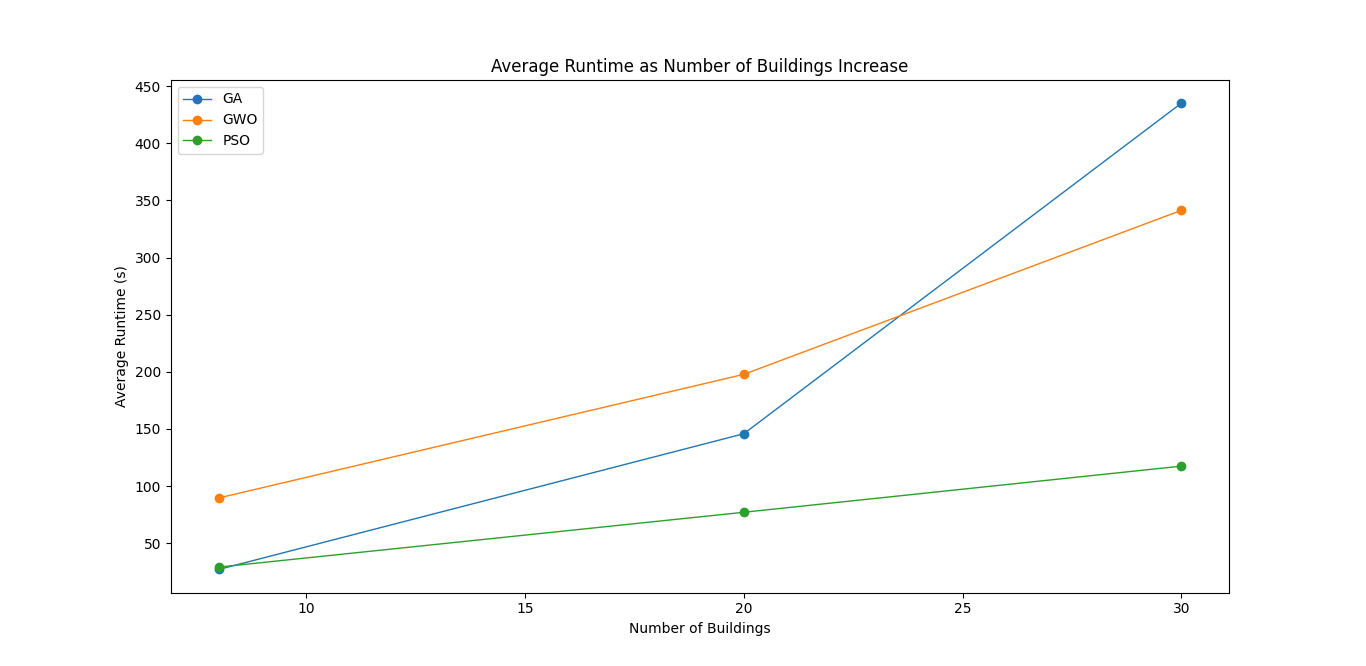
\includegraphics[scale=0.5]{./images/chap07-rd/approaches-average-runtime-over-no-of-buildings.png}
\end{adjustwidth}
\caption{The average runtime (s) of each of the approaches as the number of buildings in a data set increase.}
\label{graph-approaches-runtime-no-buildings}
\end{figure}

The genetic algorithm approach is consistently the slowest among the three problems, with PSO being the fastest. Our GWO approach was found to be the second fastest algorithm. When solving the SFLP-II, GA had an average run time of $16.3666666666667$s, compared to our approach's time and the PSO approach's $5.96666666666667$s. With mSFLP-III, the amount of time GA took to solve the problem on average was now $180.633333333333$s, while the PSO approach took $22.7666666666667$s only. Moving to mKra30a, GA further increases the amount of time now takes $557.666666666667$s on average, and the PSO approach just took $44.7$s on average. Figure \ref{graph-approaches-runtime-no-buildings} shows the impact of the number of buildings to the amount of time the approaches need on average to completely solve a problem. We can attribute this faster increase in average runtime as the number of buildings increase in the GA approach to what enables it produce better solutions on average\textemdash its local search methods. Since the local search methods perform a relatively exhaustive search in order to find a better solution, the GA will take more time to finish execution. Hence, we observe this phenomenon. This is not the case with GWO and PSO, due to the lack of local search methods. GWO may have taken a longer time compared to PSO due to the higher amount of operations that are performed in the metaheuristic. Better implementations, especially those that utilize SIMD operations, for both approaches may reduce the gap in terms of average run time between the two. However, basing from the equations in both metaheuristics, it is likely that PSO will remain faster than GWO. Further studies, however, are required to exactly determine how well each approach scales with regards to the number of buildings.

\begin{table}[h!]
\begin{adjustwidth}{-1.15in}{}
\centering
\begin{tabular}{|l|r|r|r|r|r|} 
	\hline
	\multicolumn{1}{|c|}{\multirow{2}{*}{\textbf{Problem}}} & \multicolumn{5}{c|}{\textbf{Genetic Algorithm}}                                                                                                                                                           \\ 
	\cline{2-6}
	\multicolumn{1}{|c|}{}                                  & \multicolumn{1}{c|}{\textbf{Best}} & \multicolumn{1}{c|}{\textbf{Worst}} & \multicolumn{1}{c|}{\textbf{Avg.}} & \multicolumn{1}{c|}{\textbf{Std. Dev.}} & \multicolumn{1}{c|}{\textbf{Avg. Runtime (s)}}  \\ 
	\hline
	SFLP-II                                                 & 236.266584                         & 351.084812                          & 277.8299637                        & 28.733389801383                         & 16.3666666666667                                \\ 
	\hline
	mSFLP-III                                               & 47803.047028                       & 52113.727844                        & 50309.7310666                      & 1045.05795299065                        & 180.633333333333                                \\ 
	\hline
	mKra30a                                                 & 79772.279457                       & 97487.293617                        & 88945.0482127333                   & 5158.91507488963                        & 557.666666666667                                \\
	\hline
\end{tabular}
\end{adjustwidth}
\caption{Results obtained from using the competing GA approach.}
\label{approach-ga-results}
\end{table}

\begin{table}[h!]
\begin{adjustwidth}{-1.18in}{}
\centering
\begin{tabular}{|l|r|r|r|r|r|} 
	\hline
	\multicolumn{1}{|c|}{\multirow{2}{*}{\textbf{Problem}}} & \multicolumn{5}{c|}{\textbf{Particle Swarm Optimization}}                                                                                                                                                 \\ 
	\cline{2-6}
	\multicolumn{1}{|c|}{}                                  & \multicolumn{1}{c|}{\textbf{Best}} & \multicolumn{1}{c|}{\textbf{Worst}} & \multicolumn{1}{c|}{\textbf{Avg.}} & \multicolumn{1}{c|}{\textbf{Std. Dev.}} & \multicolumn{1}{c|}{\textbf{Avg. Runtime (s)}}  \\ 
	\hline
	SFLP-II                                                 & 261.579758                         & 371.217026                          & 322.6801845                        & 32.4426073658366                        & 5.96666666666667                                \\ 
	\hline
	mSFLP-III                                               & 60132.200264                       & 68087.431686                        & 64734.7002284667                   & 1890.32624601396                        & 22.7666666666667                                \\ 
	\hline
	mKra30a                                                 & 105473.485001                      & 136518.533897                       & 120530.7167285                     & 8523.84757756761                        & 44.7                                            \\
	\hline
\end{tabular}
\end{adjustwidth}
\caption{Results obtained from our proposed PSO approach.}
\label{approach-pso-results}
\end{table}

We can further obtain insights from our results, by looking at the best solutions generated by each approach. Figures \ref{graph-approaches-best-solutions-sflp-ii} to \ref{graph-approaches-best-solutions-mkra30a} show the fitness graphs of the best solutions using the SFLP-II, mSFLP-III, and mKra30a data sets. We can observe that in the early stages of all approaches, explorations is being performed. Gradually, exploitation takes over exploration to find the best possible solution to the problems. 

Basing from the graphs we have, GA and GWO continuously exploit their abstract search space. We can attribute this behaviour to how each approach is designed. With the GA approach, remember that a local search algorithm (see Algorithm \ref{pseudocode-local-search-1}) is always being applied to the best solution the algorithm has produced (see Algorithm \ref{pseudocode-ga-approach} for details on the GA approach). Another local search algorithm (see Algorithm \ref{pseudocode-local-search-2}) is also being applied to the best solution, but only during the last 50 iterations of the algorithm. This results in the algorithm constantly exploiting the area the best solution occupies in the abstract search space and therefore further improving the best solution. Hence, the behaviour we observe in the graphs. It should be noted that we argue that the local search algorithms is what allows the GA approach to produce the best solutions on average. GWO, on the other hand, does not depend on another algorithm to fuel its exploitation. This is also a reason why it performs faster than GA. In GWO, buildings are constantly shifted around even if the number of iterations is almost near zero. However, the amount of shifting gradually reduces as the number of iterations increase (see Subsection \ref{intro-section-encircling-the-prey}, while also taking Subsection \ref{methods-section-modified-gwo} into account). This still allows buildings to find better position while reducing the risk of intersecting with other buildings. This design of our GWO approach, just with the GA approach, allows our approach to exploit the area around a local optimum and further improve the best solution it has found (along with the other solutions our approach has generated).

PSO, on the contrary, has its fitness becoming and remaining relatively stable as the number of iterations increase. This results in an almost flat line for most of the iterations in the graphs. This suggest to us that it struggles to exploit the region around its local optimum. At the start, however, it is able to explore and find good solutions. This suggests to us that

% TODO: Explain why PSO is acting poorly. 

% TODO: Remove this part.
The PSO approach has a similar characteristic that enables it to produce a continuously lowering fitness graph. In the PSO approach, as discussed before, each particle keeps track of the best position it has found. After an iteration, if a particle finds a position that is better than its personal best, then that position will replace the particle's personal. And if a particle's personal best is better than the swarm's global best, then that position/solution becomes the swarm's global best. It is this global best that is tracked in the graph. The selection procedure of the global best explains the graph of the PSO approach.

\begin{figure}[h!]
\centering
\begin{adjustwidth}{-0.45in}{}
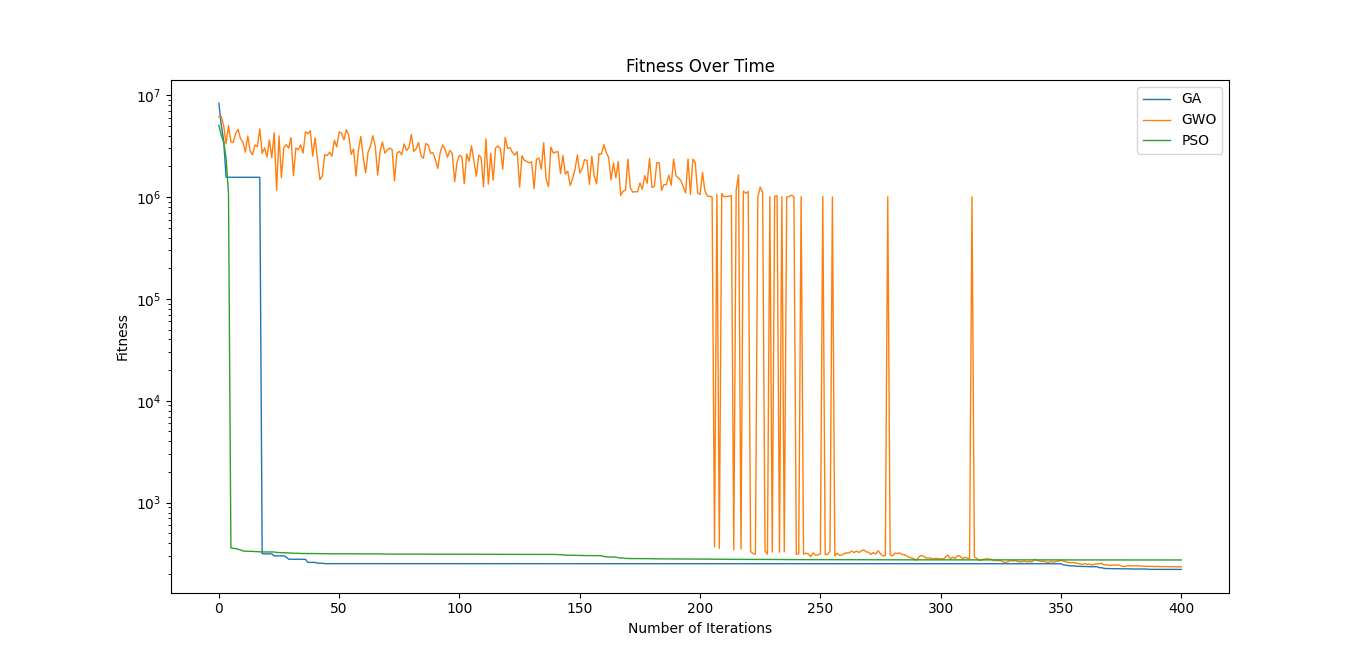
\includegraphics[scale=0.5]{./images/chap07-rd/best-fitness-over-time-sflp2.png}
\end{adjustwidth}
\caption{Fitness over time of the best solutions for the SFLP-II produced by the GA, GWO, and PSO approaches.}
\label{graph-approaches-best-solutions-sflp-ii}
\end{figure}

\begin{figure}[h!]
\centering
\begin{adjustwidth}{-0.45in}{}
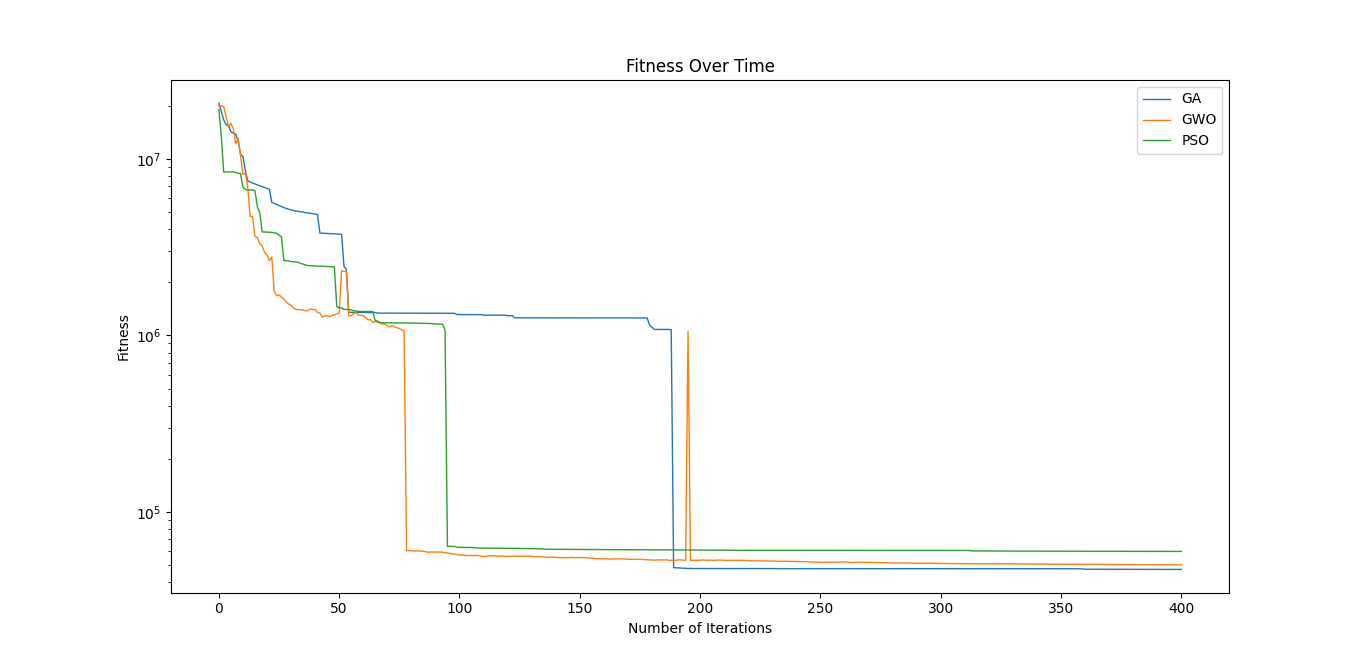
\includegraphics[scale=0.5]{./images/chap07-rd/best-fitness-over-time-msflp3.png}
\end{adjustwidth}
\caption{Fitness over time of the best solutions for the mSFLP-III produced by the GA, GWO, and PSO approaches.}
\label{graph-approaches-best-solutions-msflp-iii}
\end{figure}

\begin{figure}[h!]
\centering
\begin{adjustwidth}{-0.45in}{}
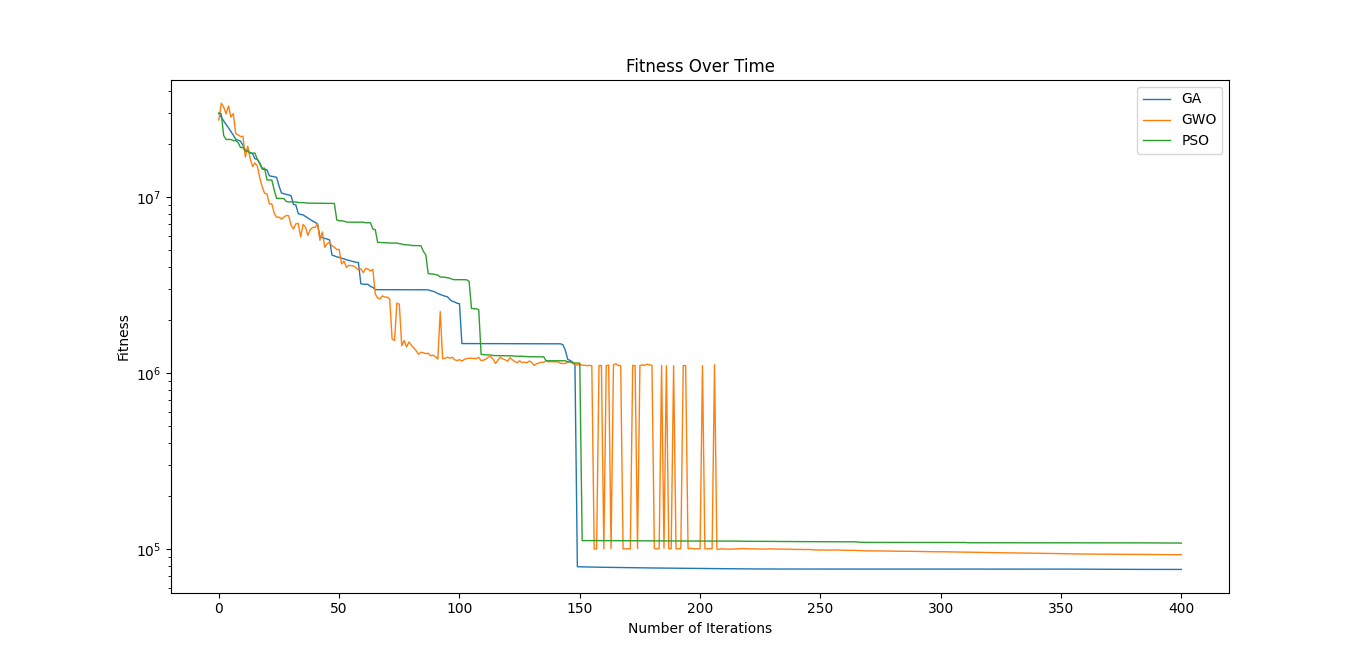
\includegraphics[scale=0.5]{./images/chap07-rd/best-fitness-over-time-mKra30a.png}
\end{adjustwidth}
\caption{Fitness over time of the best solutions for the mKra30a produced by the GA, GWO, and PSO approaches.}
\label{graph-approaches-best-solutions-mkra30a}
\end{figure}

Another avenue we can use to gather insights is through the visualization of the results produced by the approaches mentioned in this study. Figures \ref{best-results-ga} to \ref{best-results-pso} show a visualization of the best results. Notice that with the hybrid GA approach and our GWO approach, the buildings tend to clump together, which is what we want to happen, based on our objective function. For our hybrid GA approach, we can attribute the result to the local search method as well as the mutation operators as they were key to ensure that the buildings are close to each other. The crossover operator is also instrumental in achieving this result by finding combinations that will lead to the result. Our GWO approach also makes buildings clump together but not to the same degree as the GA approach, as can be observed from one building being far from the rest of the buildings in mKra30a data set in Figure \ref{best-results-gwo}. The clumping ability of our approach is attributable to how solutions are allowed to perturb their buildings to positions relatively far from the buildings positions in the best three solution initially. Eventually, our approach will decrease the distance of the buildings in a solution from the leading solutions. Remember that the leading solutions eventually become similar to each other, which help drive the reduction of the degree of building shifting. This gradually decreasing shifting of the buildings will lead to intersections from being resolved and reducing the distance of buildings from each other. The intersections are resolved by reducing the chances of buildings being to moved to a relatively further position where they would still intersect with another building, and gradually pushing intersecting buildings away from each other towards non-intersection. Note that the objective function has a lower penalty for solutions with buildings that do not significantly intersect. The decreasing shifting also encourages buildings to move towards each other due to the fact that smaller shifts have lower probability of causing buildings to intersect with one another too deeply or at all, which allows buildings to move to positions that are closer to the other buildings but without any intersections. Finally, as one can notice in Figure \ref{best-results-pso}, the PSO approach struggles to produce a solution where the buildings are clumped together. This deficiency is not necessarily clear with a small number of buildings, but it does as the number increases. We can attribute this difficulty of the PSO approach to the fact that the buildings are continuously being influenced on the same degree throughout all of the iterations by a particle's personal best and the swarm's global best. This encourages more exploitation and fewer exploitation. As a result, this reduces the chances in which buildings would be able to shift their positions by a small amount, making it more difficult for the approach to find better solutions and have buildings clump together.

\begin{figure}[h!]
\centering
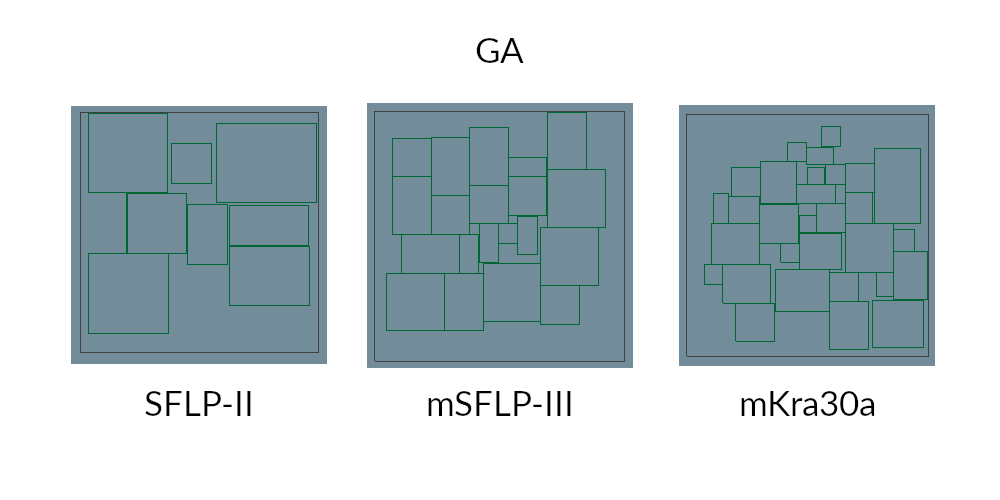
\includegraphics[scale=1.85]{./images/chap07-rd/ga-best-solutions.png}
\caption{Visualization of the best solutions produced by the hybrid GA approach for the three data sets used in this study.}
\label{best-results-ga}
\end{figure}

\begin{figure}[h!]
\centering
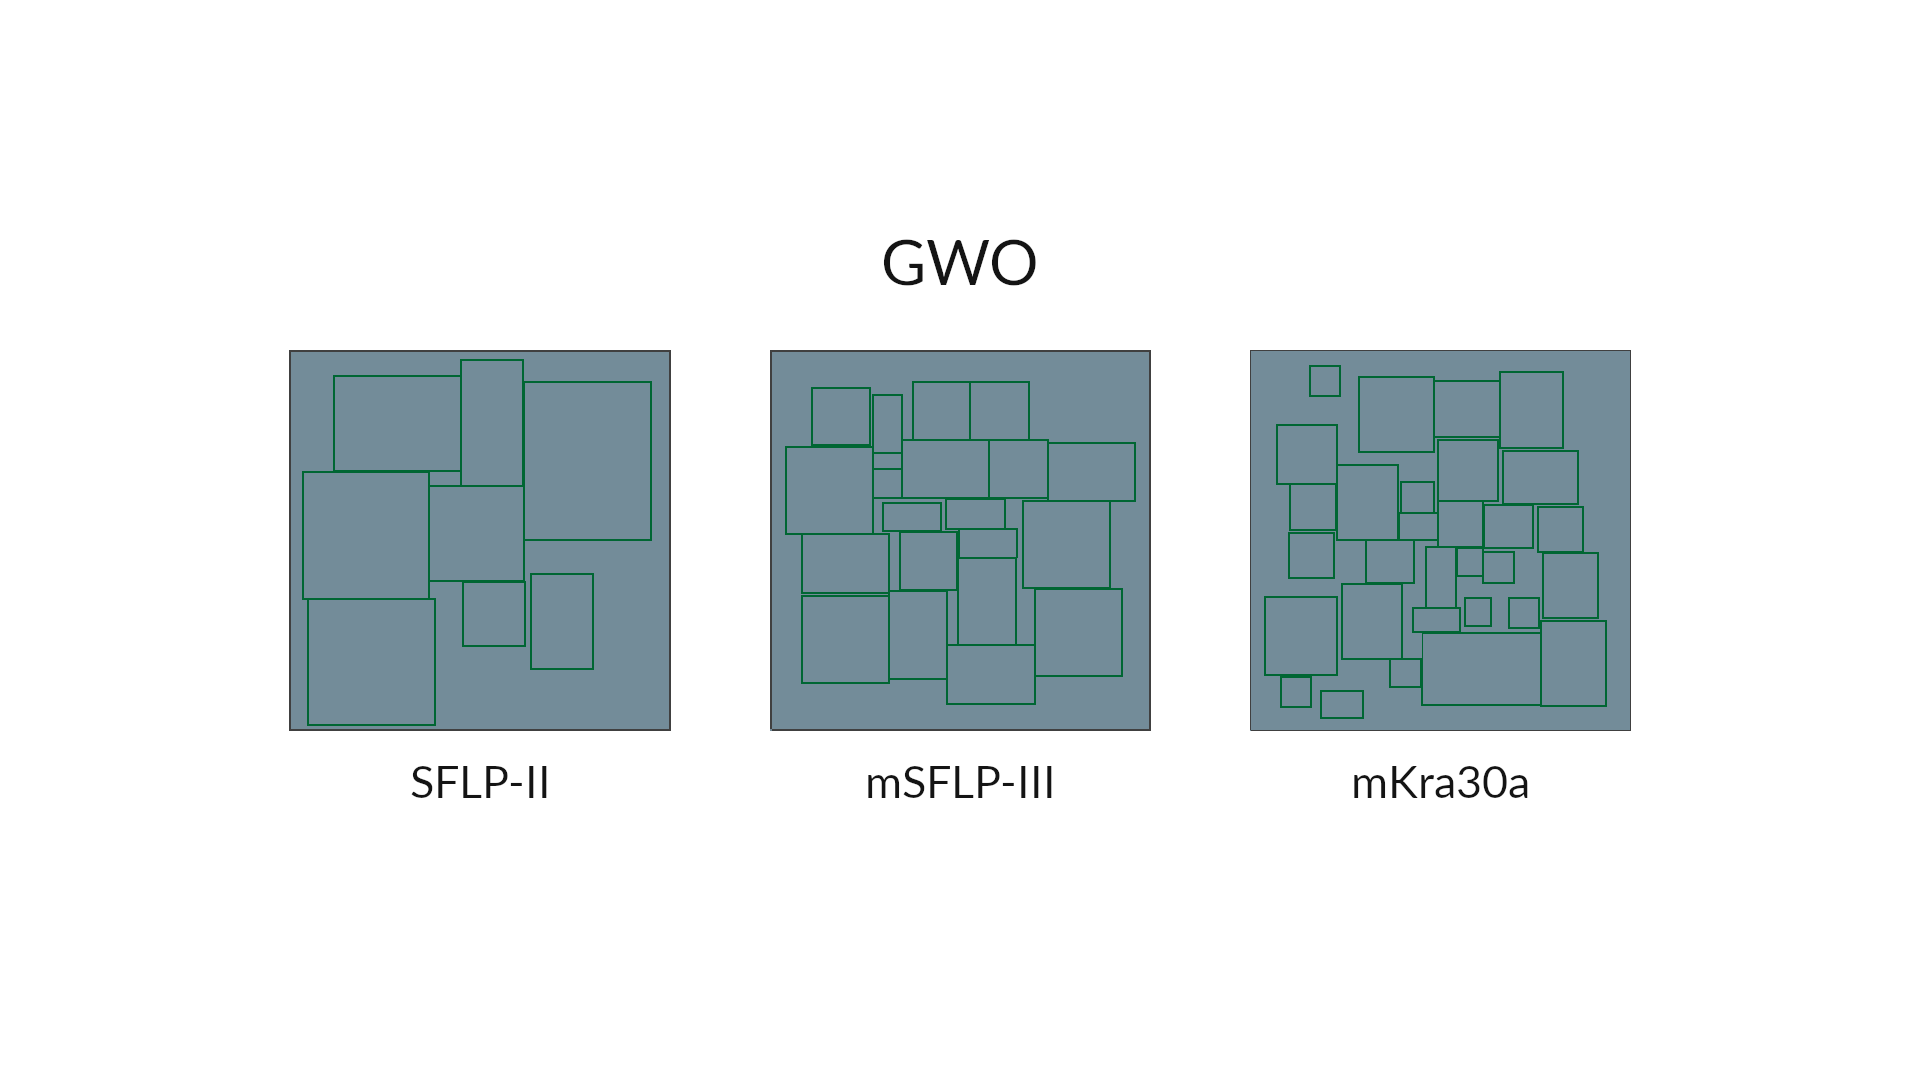
\includegraphics[scale=1.85]{./images/chap07-rd/gwo-best-solutions.png}
\caption{Visualization of the best solutions produced by our GWO approach for the three data sets used in this study.}
\label{best-results-gwo}
\end{figure}

\begin{figure}[h!]
\centering
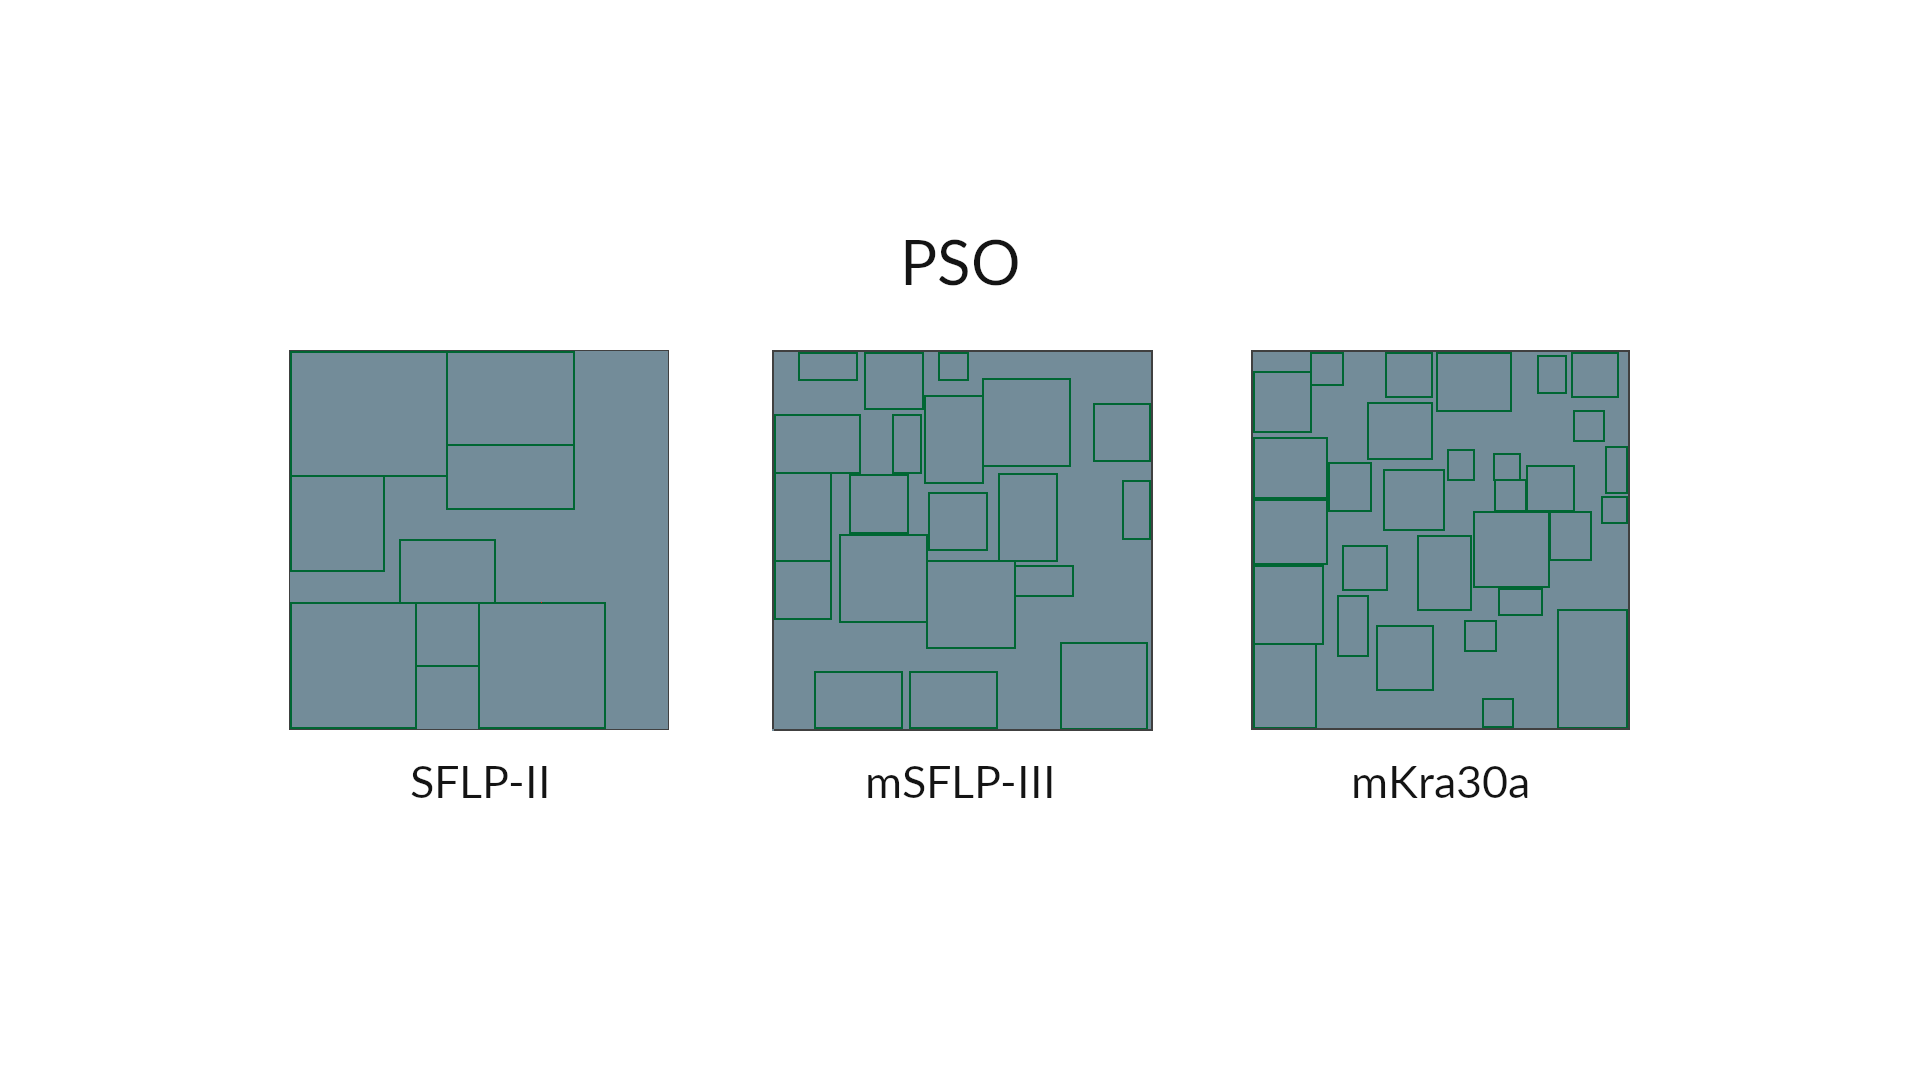
\includegraphics[scale=1.85]{./images/chap07-rd/pso-best-solutions.png}
\caption{Visualization of the best solutions produced by the PSO approach for the three data sets used in this study.}
\label{best-results-pso}
\end{figure}

For reference, Tables \ref{full-data-ga} to \ref{full-data-pso} provide the detailed numbers we have obtained in our experiments for each approach and data set. Table \ref{full-data-ga} shows the entire experiment data for our hybrid GA approach, table \ref{full-data-gwo} shows the data for our GWO approach, and lastly, table \ref{full-data-pso} shows the data for the PSO approach.

\begin{table}
\centering
\begin{adjustwidth}{}{}
\resizebox{\textwidth}{!}{\rotatebox{90}{
\begin{tabular}{|r|r|r|r|r|r|r|} 
\hline
\multicolumn{1}{|c|}{\multirow{2}{*}{Run}} & \multicolumn{6}{c|}{GA Experimental Results}                                                                                                                                                                          \\ 
\cline{2-7}
\multicolumn{1}{|c|}{}                     & \multicolumn{1}{l|}{SFLP-II} & \multicolumn{1}{l|}{Elapsed Time (s)} & \multicolumn{1}{l|}{mSFLP-III} & \multicolumn{1}{l|}{Elapsed Time (s)} & \multicolumn{1}{l|}{mKra30a} & \multicolumn{1}{l|}{Elapsed Time (s)}  \\ 
\hline
1                                          & 241.353251                   & 31                                    & 51469.406654                   & 155                                   & 76454.204788                 & 417                                    \\ 
\hline
2                                          & 260.666385                   & 27                                    & 50203.262684                   & 166                                   & 90215.278652                 & 454                                    \\ 
\hline
3                                          & 317.934947                   & 34                                    & 49903.403969                   & 159                                   & 80078.077255                 & 442                                    \\ 
\hline
4                                          & 257.12075                    & 26                                    & 51214.094765                   & 149                                   & 85424.753021                 & 453                                    \\ 
\hline
5                                          & 252.747648                   & 26                                    & 49754.550606                   & 152                                   & 85276.805458                 & 416                                    \\ 
\hline
6                                          & 291.574655                   & 27                                    & 49526.201752                   & 160                                   & 88156.523018                 & 472                                    \\ 
\hline
7                                          & 292.021864                   & 27                                    & 49669.613991                   & 157                                   & 83149.07745                  & 423                                    \\ 
\hline
8                                          & 281.474234                   & 27                                    & 51731.675354                   & 176                                   & 88411.142647                 & 413                                    \\ 
\hline
9                                          & 269.290927                   & 26                                    & 51245.732857                   & 172                                   & 90734.373741                 & 478                                    \\ 
\hline
10                                         & 269.423721                   & 27                                    & 48920.435341                   & 175                                   & 87220.602196                 & 488                                    \\ 
\hline
11                                         & 240.832309                   & 26                                    & 52856.025909                   & 212                                   & 81419.135918                 & 446                                    \\ 
\hline
12                                         & 259.251911                   & 24                                    & 49490.654926                   & 144                                   & 89084.201248                 & 498                                    \\ 
\hline
13                                         & 257.123175                   & 27                                    & 51225.387764                   & 164                                   & 82219.564217                 & 449                                    \\ 
\hline
14                                         & 232.839593                   & 26                                    & 49141.684452                   & 197                                   & 91560.704735                 & 440                                    \\ 
\hline
15                                         & 305.979567                   & 27                                    & 52062.448891                   & 161                                   & 85431.277306                 & 446                                    \\ 
\hline
16                                         & 263.951872                   & 26                                    & 51269.011093                   & 175                                   & 93689.351776                 & 451                                    \\ 
\hline
17                                         & 271.432117                   & 25                                    & 52881.041428                   & 176                                   & 85395.590744                 & 431                                    \\ 
\hline
18                                         & 278.044098                   & 33                                    & 51087.689514                   & 180                                   & 87894.849144                 & 421                                    \\ 
\hline
19                                         & 266.951438                   & 28                                    & 51001.627296                   & 171                                   & 91152.267059                 & 445                                    \\ 
\hline
20                                         & 246.816533                   & 27                                    & 50198.549866                   & 178                                   & 88895.677979                 & 471                                    \\ 
\hline
21                                         & 275.481676                   & 27                                    & 50003.058311                   & 162                                   & 87140.735931                 & 468                                    \\ 
\hline
22                                         & 353.006875                   & 26                                    & 51480.186226                   & 162                                   & 88911.361496                 & 533                                    \\ 
\hline
23                                         & 336.045243                   & 26                                    & 51068.014679                   & 182                                   & 88503.003464                 & 499                                    \\ 
\hline
24                                         & 267.427919                   & 28                                    & 53668.451469                   & 177                                   & 90751.106781                 & 487                                    \\ 
\hline
25                                         & 318.71513                    & 28                                    & 49688.022858                   & 167                                   & 87554.161316                 & 480                                    \\ 
\hline
26                                         & 239.385818                   & 31                                    & 50890.728996                   & 161                                   & 89753.353699                 & 516                                    \\ 
\hline
27                                         & 235.181557                   & 27                                    & 51466.78817                    & 160                                   & 92770.250797                 & 431                                    \\ 
\hline
28                                         & 256.815948                   & 27                                    & 47177.914444                   & 159                                   & 93206.425659                 & 443                                    \\ 
\hline
29                                         & 329.646141                   & 27                                    & 50171.089684                   & 146                                   & 84805.798279                 & 473                                    \\ 
\hline
30                                         & 255.073269                   & 27                                    & 49837.797424                   & 151                                   & 96215.108131                 & 381                                    \\ 
\hline
\multicolumn{1}{|l|}{Average}              & 274.120352366667             & 27.3666666666667                      & 50676.8183791                  & 166.866666666667                      & 87715.8254635                & 455.5                                  \\ 
\hline
\multicolumn{1}{|l|}{Std. Dev}             & 31.3302957404409             & 2.17324377503931                      & 1325.4427345102                & 14.6775299372024                      & 4281.86238995314             & 33.3639801644497                       \\
\hline
\end{tabular}}}
\end{adjustwidth}
\caption{The entire experiment data we have collected using our hybrid GA approach.}
\label{full-data-ga}
\end{table}

\begin{table}
\centering
\begin{adjustwidth}{}{}
\resizebox{\textwidth}{!}{\rotatebox{90}{
\begin{tabular}{|r|r|r|r|r|r|r|} 
\hline
\multicolumn{1}{|c|}{\multirow{2}{*}{Run}} & \multicolumn{6}{c|}{PSO Experimental Results}                                                                                                                                                                         \\ 
\cline{2-7}
\multicolumn{1}{|c|}{}                     & \multicolumn{1}{l|}{SFLP-II} & \multicolumn{1}{l|}{Elapsed Time (s)} & \multicolumn{1}{l|}{mSFLP-III} & \multicolumn{1}{l|}{Elapsed Time (s)} & \multicolumn{1}{l|}{mKra30a} & \multicolumn{1}{l|}{Elapsed Time (s)}  \\ 
\hline
1                                          & 318.852793                   & 30                                    & 64984.15004                    & 76                                    & 126400.957298                & 130                                    \\ 
\hline
2                                          & 322.977083                   & 28                                    & 65613.267347                   & 81                                    & 121843.241837                & 115                                    \\ 
\hline
3                                          & 319.688772                   & 27                                    & 66182.148331                   & 77                                    & 131064.62114                 & 117                                    \\ 
\hline
4                                          & 382.774055                   & 29                                    & 65321.947243                   & 74                                    & 123193.080185                & 109                                    \\ 
\hline
5                                          & 328.181972                   & 26                                    & 68316.333054                   & 90                                    & 113509.606079                & 116                                    \\ 
\hline
6                                          & 273.754488                   & 27                                    & 63051.351074                   & 80                                    & 126382.984985                & 104                                    \\ 
\hline
7                                          & 277.929458                   & 35                                    & 64844.383484                   & 80                                    & 118793.658676                & 113                                    \\ 
\hline
8                                          & 333.791855                   & 29                                    & 62119.790359                   & 78                                    & 116690.745407                & 115                                    \\ 
\hline
9                                          & 331.588456                   & 25                                    & 62520.697372                   & 81                                    & 112328.409836                & 114                                    \\ 
\hline
10                                         & 312.062043                   & 28                                    & 60370.992424                   & 70                                    & 125547.949913                & 117                                    \\ 
\hline
11                                         & 347.300041                   & 26                                    & 63191.887421                   & 74                                    & 128467.742325                & 111                                    \\ 
\hline
12                                         & 276.72711                    & 29                                    & 66079.518539                   & 75                                    & 115259.262817                & 123                                    \\ 
\hline
13                                         & 346.501261                   & 38                                    & 68433.641548                   & 72                                    & 120682.394836                & 123                                    \\ 
\hline
14                                         & 324.057936                   & 29                                    & 59673.997963                   & 73                                    & 115606.839714                & 136                                    \\ 
\hline
15                                         & 294.477526                   & 33                                    & 65232.604935                   & 77                                    & 107996.773666                & 135                                    \\ 
\hline
16                                         & 354.944439                   & 28                                    & 62623.302681                   & 77                                    & 117466.287628                & 119                                    \\ 
\hline
17                                         & 278.580433                   & 25                                    & 63571.512451                   & 78                                    & 119787.763885                & 111                                    \\ 
\hline
18                                         & 373.62812                    & 25                                    & 65604.954414                   & 73                                    & 121933.62674                 & 111                                    \\ 
\hline
19                                         & 277.326199                   & 27                                    & 60121.135582                   & 71                                    & 120619.96003                 & 128                                    \\ 
\hline
20                                         & 312.888415                   & 26                                    & 65799.8442                     & 77                                    & 114528.809418                & 112                                    \\ 
\hline
21                                         & 349.500618                   & 28                                    & 62835.800159                   & 86                                    & 123371.321442                & 113                                    \\ 
\hline
22                                         & 324.432381                   & 30                                    & 67968.856182                   & 80                                    & 125755.185791                & 107                                    \\ 
\hline
23                                         & 259.640869                   & 29                                    & 61263.364929                   & 77                                    & 114837.336021                & 109                                    \\ 
\hline
24                                         & 324.809072                   & 28                                    & 64277.566399                   & 78                                    & 119911.446892                & 114                                    \\ 
\hline
25                                         & 315.892269                   & 30                                    & 63997.453415                   & 72                                    & 130395.024284                & 101                                    \\ 
\hline
26                                         & 367.985685                   & 31                                    & 62791.55909                    & 73                                    & 126777.9534                  & 109                                    \\ 
\hline
27                                         & 306.720735                   & 37                                    & 66069.317642                   & 77                                    & 116590.569717                & 132                                    \\ 
\hline
28                                         & 373.704857                   & 29                                    & 65694.84201                    & 77                                    & 131275.843658                & 145                                    \\ 
\hline
29                                         & 288.776388                   & 30                                    & 67406.459572                   & 76                                    & 118132.533211                & 120                                    \\ 
\hline
30                                         & 339.280296                   & 30                                    & 62731.473629                   & 81                                    & 126570.733612                & 113                                    \\ 
\hline
\multicolumn{1}{|l|}{Average}              & 321.292520833333             & 29.0666666666667                      & 64289.8051163                  & 77.0333333333333                      & 121057.4221481               & 117.4                                  \\ 
\hline
\multicolumn{1}{|l|}{Std. Dev}             & 32.8103600821748             & 3.20488133443597                      & 2356.26248290771               & 4.29501180868943                      & 5981.21601161922             & 10.1526283330459                       \\
\hline
\end{tabular}}}
\end{adjustwidth}
\caption{The entire experiment data we have collected using our PSO approach.}
\label{full-data-pso}
\end{table}

The performance of the GA approach in this study is definitely noteworthy. It produces the best solutions on average among the three approaches. However, based on the results, the GA approach does not scale well as the number of buildings increase, compared to our approach and the PSO approach. PSO definitely shows the best average runtimes. However, it produces the worst average fitness. For faster speed, we traded performance. This is where our approach shines. Our approach is the second best when it comes to solution quality as the problem scales higher. It is also the second best in terms of speed. This shows to us that our GWO approach provides a balance between speed and performance. Our approach also requires only a few parameters. We argue that this will simplify and speed up experimental setups and configuration in later studies and applications. Importantly, the results also indicate that there is promise in further exploring the applicability of the grey wolf optimization algorithm in solving the facility layout problem.

% TODO: Mention in the methods chapter that the best solution is always kept in our GWO approach.
